
%%%%%%%%%%%%%%%%%%%%%%% file typeinst.tex %%%%%%%%%%%%%%%%%%%%%%%%%%%%%%
%
% This is the LaTeX source for the instructions to authors using
% the LaTeX document class SVMultln with class option 'lnicst'
% for contributions to the Lecture Notes of the Institute for
% Computer Sciences, Social-Informatics and
% Telecommunications Engineering series.
% www.springer.com/series/XXXX       Springer Heidelberg 2007/08/05
%
% It may be used as a template for your own input - copy it
% to a new file with a new name and use it as the basis for
% your article. It contains a few tweaked sections to demonstrate
% features of the package, though.
%
% If you have not much experiences with Springer LaTeX support,
% you should better use the special demonstration file "lnicst.tex"
% included in the LaTeX package for LNICST as template.
%
%%%%%%%%%%%%%%%%%%%%%%%%%%%%%%%%%%%%%%%%%%%%%%%%%%%%%%%%%%%%%%%%%%%%%%%%
\documentclass[lnicst,sechang,a4paper]{svmultln}
\usepackage{amssymb}
\setcounter{tocdepth}{3}
\usepackage{graphicx}

\usepackage{url}
\usepackage[pdfpagelabels,hypertexnames=false,breaklinks=true,bookmarksopen=true,bookmarksopenlevel=2]{hyperref}

\usepackage{makeidx}

\usepackage{graphicx}
\usepackage{multirow}
\usepackage{textcomp}
\usepackage{color}
\usepackage{caption}

\begin{document}

\mainmatter  % start of an individual contribution

% first the title is needed
\title{VMGuards:Fine-grained Software Tamper\\ Proofing System
for PVM-Based \\ Code Obfuscation}

% a short form should be given in case it is too long for the running head
\titlerunning{VMGuards: A PVM-Based Software Tamper Proofing}

% the name(s) of the author(s) follow(s) next
%
% NB: Chinese authors should write their first names(s) in front of
% their surnames. This ensures that the names appear correctly in
% the running heads and the author index.
%
\author{Meiling Chen$^\dag$
\and Zhanyong Tang$^\dag$\thanks{Correspondence should be addressed to Zhanyong Tang.Email:zytang@nwu.edu.cn}
\and Zhaohui Hao$^\dag$
\and Xiaoqing Gong$^\dag$
\and\\ Dingyi Fang$^\dag$
\and Xiaojiang Chen$^\dag$
\and Zheng Wang$^\ddag$}  %
\authorrunning{VMGuards: A PVM-Based Software Tamper Proofing}
% (feature abused for this document to repeat the title also on left hand pages)

% the affiliations are given next
\institute{$^\dag$School of Information Science and Technology,\\ Northwest University, Xi��an, 710127, P.R. China.
\\$^\ddag$School of Computing and Communications, \\ Lancaster University, Lancaster, England.\\
%\\
%\url{http://www.springer.com/series/7911}
}

%
% NB: a more complex sample for affiliations and the mapping to the
% corresponding authors can be found in the file "lnicst.dem",
% that is contained in the LNICST LaTeX support package.
%

\toctitle{VMGuards:Fine-grained Software Tamper Proofing System for PVM-Based Code Obfuscation}
\tocauthor{Authors' Instructions}
\maketitle


\begin{abstract}
Software tamper-proofing mechanisms have been increasingly proposed to defend against code-tampering attacks.Process-level Virtual Machines (PVMs) is emerging as a viable method, which works by implementing code obfuscation to protect programs code intergrity statically and checking them at runtime. Coarse-grained enforcements of PVMs that transform and restore the key code segment of the original program into a new section have been shown to be ineffective. However, with advanced tools and techniques, an adversary can locate where and what the new section is and contains, also he can get the organization structure and the execution principle of the new section through static or/and dynamic analysis.

As a result, a lot of recent efforts have focused on fine-grained enforcement of PVMs self-security as it was originally proposed. In this work ,we show a fine-grained mechanism of PVMs, which takes the virtual machines self-security into account, uses to detect tamper behavior at run time to a PVM-protected program. We designed tamper-proofing instruction (TPI) and anti-debug instruction (ADI) based on the idea of guards and anti-debug techniques, to improve the security of the normal virtual instruction during the execution of the protected software. We implemented a Proof-of-Concept prototype, VMGuards, to demonstrate our idea, while incurring only modest performance overhead (17\%) and requiring a small amount of changes to the protected code. Key contributions of VMGuards are a fine-grained architecture for securing PVM and a method for generating  TPI\&ADI from binary code.
\keywords{Software tamper-proofing, Process-level virtual machine protection, Tamper-proofing instruction, Anti-Debug Protection}
\end{abstract}


\section{Introduction}

Tamper is one of the three most major problems encountered in the process of software protection. To an adversary, he will utilize reasonable tools to modify an application, and then put these after-modified applications into use in an unexpected way. However, the value contained in and protected by software is huge. According to the Business Software Alliance and the International Data Corporation, malware problems associated with unlicensed software cost organizations nearly \$500 billion in 2014\cite{bus}. The resources and later maintenances for a software are difficult to describe through numbers. Nevertheless, most software are failed in the market at present, the damages the software developers'benefits badly.

Software tamper proofing technique is a general term of software protection techniques, which is used to prevent an application from unauthorized modifying by means of software or hardware. In recent years, researches on process-level virtual machines (PVMs) have become one hotspot in the field of software tamper-proofing protection\cite{vir}.

The basic idea behind virtual machine is, transforming the executable code based on x86 assemble system into bytecode, then inserting a specific designed virtual machine interpreter (called VMInterpreter) into the application, which is used to interpretive executing the transformed bytecode, to prevent the original code from easily reverse engineering or tampering. At run time, the VMInterpreter will take over the execution when it executes to the key code segment. Otherwise, the program will be normally executed.

In order to protect key code segment, many of PVMs transform and restore the crucial code part of the original program into a new section. However, the existing process-level virtual machine software protection scheme cannot ensure the virtual instructions'self-security. With advanced tools and techniques, an adversary can locate where and what the new section is and contains, he can also get the organization structure and the execution principle of the new section through static or/and dynamic analysis.

Prior work has widespread employed software guards to dynamically protect the program in software tamper-proofing area\cite{prot}. However, these implementations are either simple structure or high overhead\cite{def}.Owing to the theory of comparison, a comparable value will be hidden somewhere in the program, an adversary can bypass the protection if he has successfully located the cmp instructions.

Moreover, a number of software protection schemes only provide a partial solution and suffer from an impractical overhead. The Proteus\cite{pro} system brings 50X-3500X overheads, which are too high for most programs. Remote tamper-proofing schemes\cite{pio} are widely used in embedded devices, but they require strict Quality-of-Service guarantees\cite{on}. A practical scheme should not bring in so much significant overhead, or developers will be unwilling to deploy such measures on a large scale.

This work proposed a novel method for software tamper-proofing scheme, VMGuards, on the basis of previous works on PVMs, which takes the virtual machines self-security into account, used to detect tamper behavior at run time to a PVM-protected program. We designed tamper-proofing instructions (TPI) based on the idea of guards to maintain the integrity of a fixed length code and at the same time introduces anti-debug instruction (ADI) based on the anti-debug techniques to guarantee an unharmed host.

This paper makes the following contributions:

\begin{description}
  \item[1)] \textbf{Tamper-proofing Instruction.} It designs a Tamper-Proofing Instruction (TPI) to detect tamper behaviour during program execution to ensure the normal virtual instructions'security. These TPIs can only be recognized by our PVM system and totally similar with the normal virtual instruction. On the other hand, we designed these TPIs with a circulation form, to keep each TPI safe from modifying.
  \item[2)] \textbf{The Concept of Anti-debug protection.} It presents the concept of anti-debug protection, applying five detection and two response mechanisms to detect and make sure that the outside environment of the program is unharmed.
  \item[3)] \textbf{Evaluating the performance of VMGuards.} It designs and implements VMGuards, and has experimented it by a set of practical software cases, the experiment results show that VMGuards can be used to protect software, and the overhead can be accepted.
\end{description}

The remainder of the paper is organized as follows. Section2 we describe the threat model in which a program executed. Section3 gives an overview of VMGuards. The concept of TPI and ADI are explained in Section4 and Section5. And in Section6 we evaluate and discuss the performance and overhead of VMGuards. Previous works in software tamper-proofing area are discussed in Section7. Finally, in Section8 presents our conclusions.

\section{Threat model}

VMGuards's threat model is the same as the strong model in the original Tamper Proofing\cite{pio}. An attacker is modeled as a concurrent user hostile environment, debugging tools which can simulator to execute and even modify the protected program. The attacker can read and write any memory. Skype, for example, the popular VoIP tool\cite{sil}, was cracked by a debugger to get the key-code segment information in memory base. Therefore, in this model, even the OS can be modified to return a negative result.  What is more, the adversary can simulate a hardware to return a``forged true-resul'' to the application. As a result, we assume that the hardware and the software on a host machine are potentially vicious, and all protected programs (including the ones on the host machine) are the targets of the adversary. 

In fact, we assume that it's a white-box attack for the adversary. That's to say, the adversary can detect, modify or forge every information on the host machine. So with enough time and resources, the adversary can successfully detect and modify any protected program. Moreover, human adversaries can hardly resolve large data set problems, they have to rely on automatic analysis tools to perform malicious behaviors. At this point, as a protector who needs to increase the overhead or disable the mal-tools which an adversary tries to crash the protected program by every means.

\section{Overview of VMGuards}
From Section2, we have already known the threat model. Next we need to be familiar with the framework of our VMGuards before we introduce the design of the TPI and ADI. Basically, we divide virtual machine into two categories, the most common one is System-level Virtual Machine, such as VMWare Workstation, VirtualBox, Xen, and these SVM provide a complete system environment for the OS and the related applications\cite{virt}. The other one is Process-level Virtual Machine, which is more suitable for software protection, for it virtualizes a single user-level application.

Therefore, on the basis of Process-level Virtual Machine, we proposed our PoC-VMGuards. VMGuards provides a decryption tamper-proofing mechanism to the encrypted program instructions at runtime.

\begin{figure}[htb]%ͼ1
    \centering
    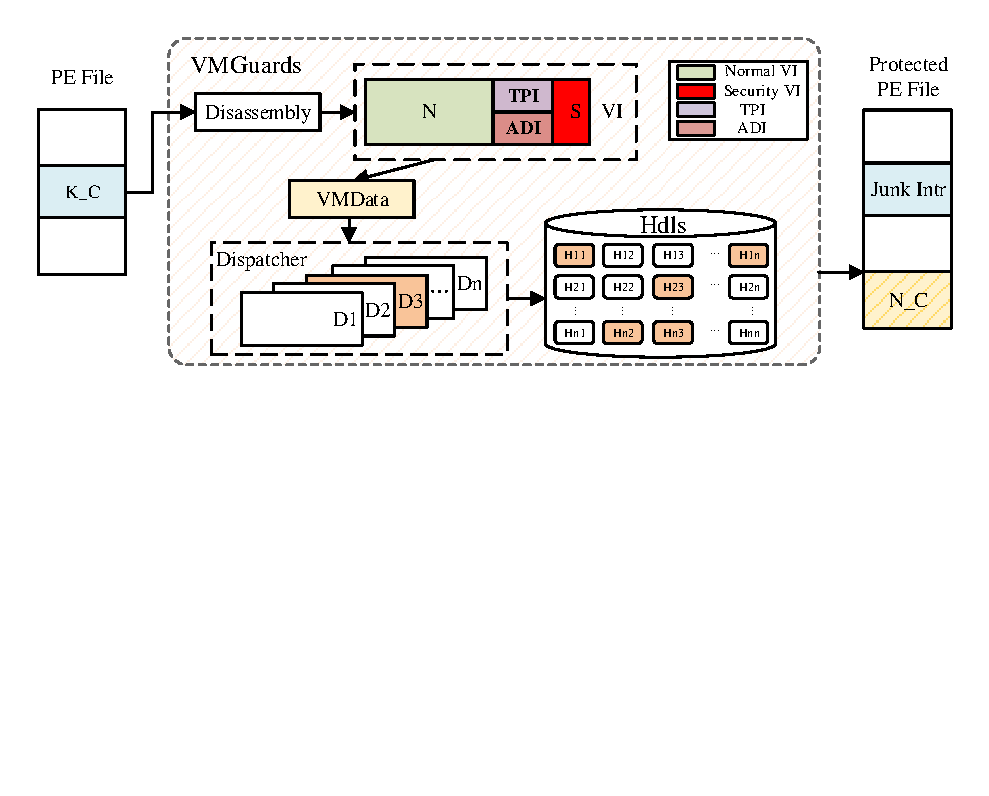
\includegraphics[width=0.9\columnwidth]{figure/framework.pdf}
    \caption{The framework of VMGuards.TPI and ADI are two kinds of security instruction, which can ensure the virtual instructions'self-security.}\label{fig:Fig.1}
\end{figure}

Our VMGuards works as follows: first, it will control and disassemble the program's instructions during startup. The disassembled instructions then be transformed to a mid-expression, we call it Virtual Instruction (VI). Next, control will transfer to the new section, until the new section is completely executed. Lastly, the new section will retrieve the control to normal execution, till the program finished. Figure.~\ref{fig:Fig.1} shows the main framework of our VMGuards. In the figure, K\_C for key code segment which represents the crucial code part of the program such as the key algorithm, the authorization information used in the program, after protection the segment will be filled up with some junk or useless code, N\_C for new code section where stored the after-protected key code, VI for virtual instruction which will be introduced next. The components will be introduced one by one.

\subsection{Disassmebly}

As far as we know, there are two basic disassembly techniques\cite{flow}: linear disassembly and recursive disassembly. The former begins by disassembling the very first instruction of the program. Once an instruction at an address is disassembled, and is decided to have a length of l bytes, disassembly proceeds to the instruction starting at address addr+l. This process continues to the end of the program. Linear disassembly can be confused by ``gaps'' in code that consist of data or alignment-related padding. These gaps will be interpreted by linear disassembly as instructions and decoded, resulting an erroneous disassembly.

The latter uses a different strategy. It starts with a set of code entry points specified in the binary. For an executable, there may be just one such entry point specified, but for shared libraries, the beginning of each exported functions is specified as well. Unlike linear disassembly, recursive disassembly does not get confused by gaps in code, and hence does not produce incorrect disassembly. Nevertheless, it fails to disassemble code that is reachable only via Indirect Control Flow (ICF) transfers.

Our approach combines linear disassembly and recursive disassembly. We utilize linear disassembly to make sure the integrity of the disassembly result and guarantee the correctness of the disassembly result by recursive disassembly.

\subsection{Virtual Instruction}

After disassembled all instructions, we need to transform these disassembled instructions into a mid-expression\cite{pro}, Virtual Instruction (VI), so that they can only be recognized by our VMGuards when the protected program is executed. Moreover, we have the freedom to design our own VI, this leaves us many choices to make. In this paper, we designed VI to simplify the correspondence between the original instructions and the Handlers, making the design of VMGuards more concise. While the relationships between the original instructions and virtual instructions, and virtual instructions and Handler are many-to-many, this will increase the difficulty of reverse engineering. The virtual instructions, however, are not stored in the protected program.

In our VMGuards, there are three main principles to design a reasonable VI sets. First of all, completeness, that's to say, the designed VI must be able to interpret all x86 instructions; Secondly, complexity, a reasonable complexity can lead to a many-to-many relationship, otherwise VI is redundant; Last but not least, functionality, every virtual instruction must has a clearly defined meaning, it can precisely guide an x86 instruction to a certain Handler sequence.

Tamper-proofing instructions and Anti-debug instructions are two most designed security virtual instructions. The former is designed to keep the key code segment of the program from tampering, and the latter can make sure that there are no reverse engineering tools exist on the host machine during the program execution. That's to say, by these two security instructions we can, on one hand, keep the program inner safe, on the other hand, prevent the outside execution environment of the program from malicious tools. The following section4 and section5 will focus on these two virtual instructions, more details will be introduced one by one.

\subsection{Handler Set}

Handler set is short for Hdls. Hdls is consist of multiple Handlers. Handlers are some small instruction segments, and in our design, there are two types of Handlers, one is parameter-free, and the other contains one or more parameters. In one Handler, it may contain one or some of the following operations: mathematical operation, conditional jump operation, assignment operation and special operation. To be clear, in this paper, the Handler is not the common handle in Windows, it's a small piece of program can be invoked by the Dispatcher (will be introduced in the following section), which is used to interpret the original x86 instructions. In other words, every original x86 instruction can be interpreted by several Handlers through a mapping relationship with virtual instructions. That is to say, original x86 instruction firstly should be mapped to virtual instructions, then be interpreted by several Handlers. Figure.~\ref{fig:Fig.2} shows the mapping relationship of the three elements.

As we can see, if we assume the x86 instruction in the first block be the key code segment of the program, at the first step they will be transformed to VI and then mapped to Handlers.

\begin{figure}[htb]%ͼ2
    \centering
    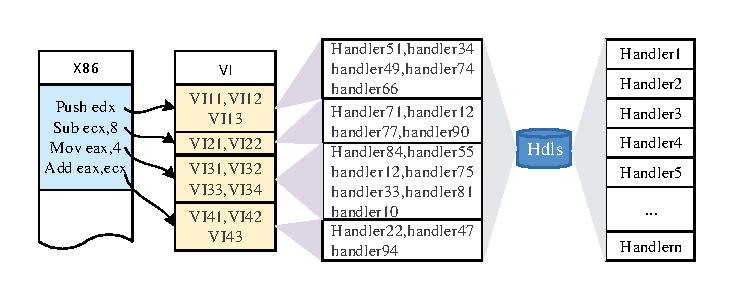
\includegraphics[width=0.9\columnwidth]{figure/x86.pdf}
    \caption{Every original x86 instruction maps to several sets of Handlers.}\label{fig:Fig.2}
\end{figure}

\subsection{Dispatcher}

Like buses have dispatching centers, our VMGuards have Dispatchers, which are used to read and decrypt the VMData (will be introduced in the following section), after decryption the plaintext will be used to calculate the corresponding Handlers'addresses by certain algorithm, and then the program will jump to the accurate address to execute. At this point, we can see that the Dispatcher is a crucial component of the VMInterpreter, which controls the dispatching process to Handler.

So far, so many researches about PVM have targeted on improving the structure of Dispatcher, and currently we can classify the existing structures into three categories: (1) Centralized model; (2) Chained model; and (3) Hybrid model. In this paper, we prefer to employ the third one. Because it's easy to reverse engineering the centralized model to find the only one Dispatcher, further to locate all the Handlers which called by the Dispatcher. For the chained model, it's one way in and one way out, Handles in chained model Dispatcher are called by an offset from one to another, as long as the adversary find the jmp instruction behind every Handler, he can get all Handlers, furthermore reverse engineering the whole program.

That is the reason why we choose to combine the Centralized model and the Chained model together to improving the security of Dispatcher's structure. There are following advantages by improving the design of the Dispatcher's structure. Firstly, an adversary cannot gather the whole dispatching procedure through only one fixed Dispatcher's address; Secondly, we designed all these Dispatchers similar to the normal Handlers, and after a Handler is executed, it randomly returns to one of these Dispatchers or Handlers, so as an adversary, he cannot easily figure it out which one is Dispatcher and which one is Handler. Figure~\ref{fig:Fig.3} gives a sketch map of the structure.

\begin{figure}[htb]%ͼ3
    \centering
    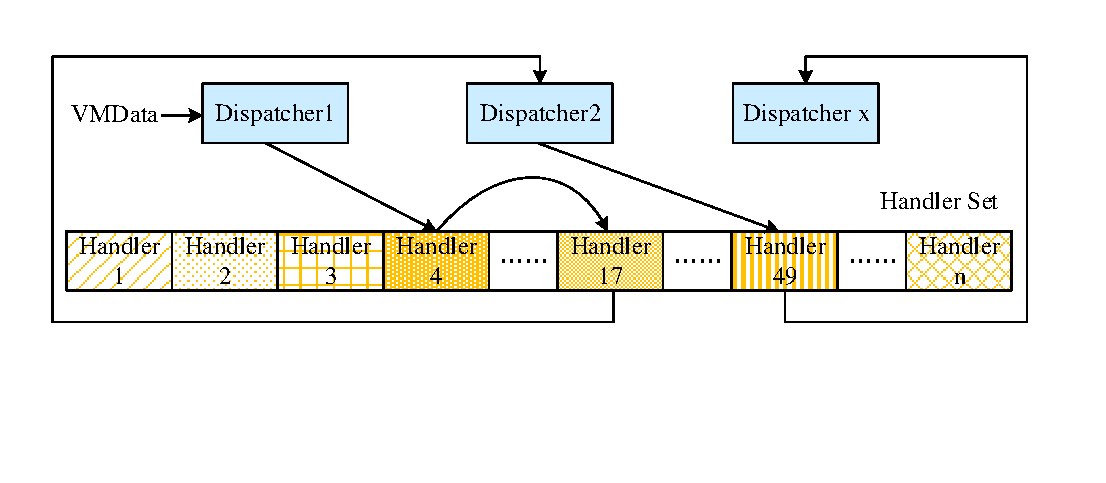
\includegraphics[width=0.9\columnwidth]{figure/dispatcher.pdf}
    \caption{The structure of hybrid model Dispatcher}\label{fig:Fig.3}
\end{figure}

\subsection{VMData}

As we can see from figure~\ref{fig:Fig.3}, VMData is an encrypted data used to drive the Handler to execute, and it's an encrypted being executed Handler sequence. More specifically, the VMInterpreter chooses Handler to execute based on the VMData read in the Dispatcher. Seeing from subsection 3.3, there are two kinds of Handler, to the one that contains one or more parameters, VMData also provide an encrypted data to the parameters to further obfuscate the Handler number and the parameters.

So many crucial information, VMData included, will be used by the VMInterpreter, that's why we usually protect them with an encryption mechanism. Correctly generating the VMData is the key to accurately dispatching the Handler, therefore, the specific meaning of the VMData is closely related to the Dispatcher.


\section{Tamper-Proofing Instruction}

The concept of guards was first proposed by Chang and Atallah\cite{prot} as a tamper-proofing mechanism. Part of this scheme is a checking primitive-code checksum, which calculates the checksum of a protected code segment. Existing researches on software guards have gained so much successes\cite{dyn,obl,sof,uni}. However, these implementations is either simple structure or high overhead. As we know, in Chang's scheme, guards is said that reading the code segment tends to stick out as an atypical operation during execution, the adversary then can usually pin-point the checks by setting breakpoints or examining the code. The main drawback of guards-net is that the complexity will result in higher overhead and longer execution time, this is the disadvantage to debug and optimize the program for the software developers; moreover, the function of every guard is the same, and all guards are run in the host process. Thus, an adversary can locate one guard by debugging the process, then he can disable them all.

\begin{figure*}[htb]
\centering
\begin{minipage}[b]{0.45\linewidth}
\centering
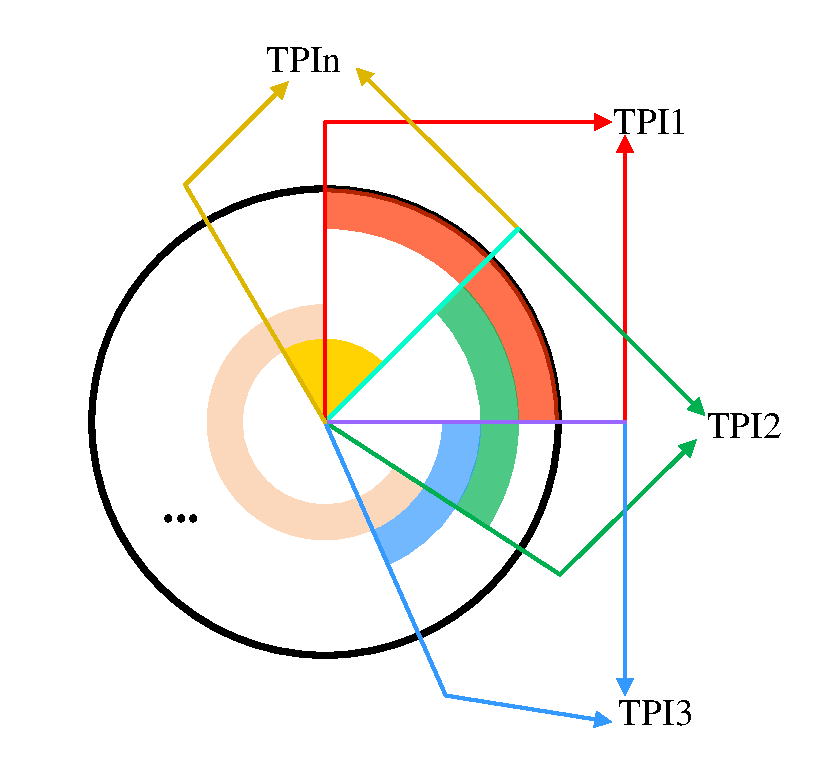
\includegraphics[width=2.1in]{figure/ring.pdf}
\captionsetup{justification=centering}
\caption{The organization of TPI-Ring.To make sure every sensitive area at least has three TPI Handler protecting it.}
\label{fig:Fig.4}
\end{minipage}%
\begin{minipage}[b]{0.55\linewidth}
\centering
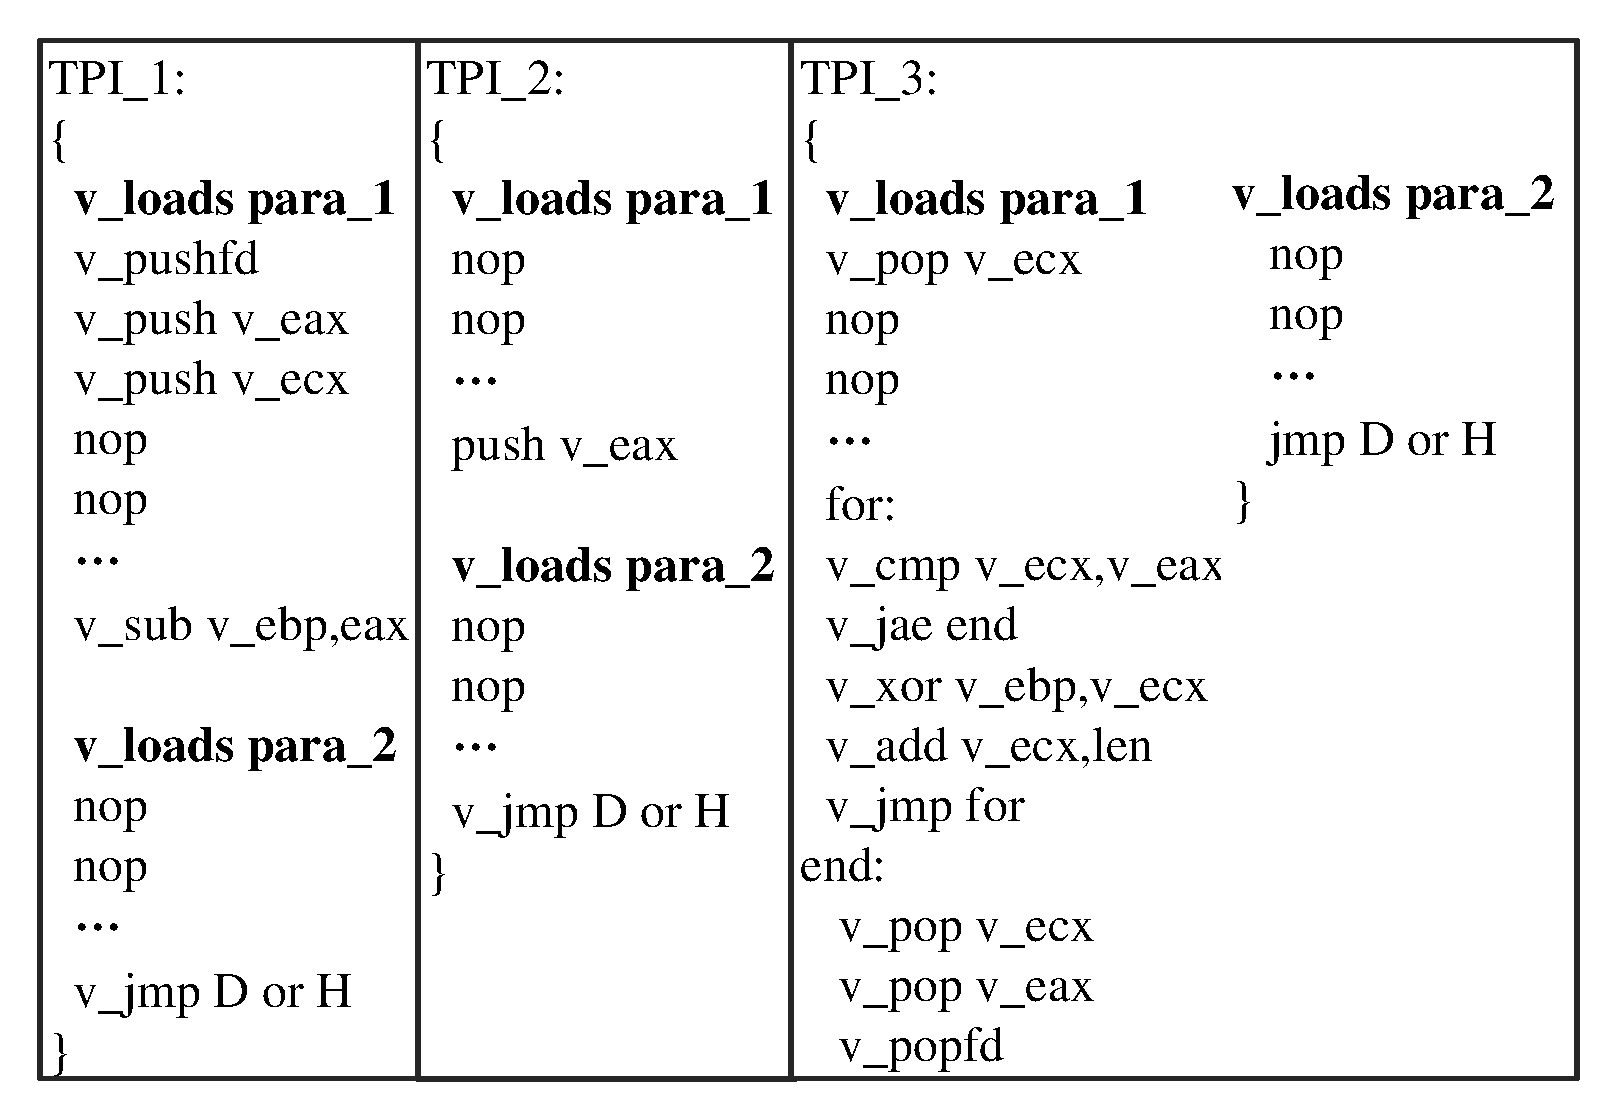
\includegraphics[width=2.5in]{figure/handlers.pdf}
\captionsetup{justification=centering}
\caption{A TPI consists of three different handlers. TPI\_a,to load the checksum and operate it with EBP. TPI\_b,to load the start address. TPI\_c,to load the end address and restore EBP.}
\label{fig:Fig.5}
\end{minipage}
\end{figure*}

In this paper, we introduced Tamper-Proofing Instruction, TPI for short, which is consist of existing Handlers, to achieve the same function as guards, but presents as normal Handlers. By this very design, on one hand, the key code segment of the program is detected and protected by TPI, on the other hand, the structure of TPI Handler will be obfuscated with normal Handlers, making it troublesome to recognize which Handler determines the function of TPI. Furthermore, we designed multiple kinds of TPI to against the attack that the adversary can remove all checkpoints just from one, and every two TPI are crossed with each other to make sure that when an adversary can locate and remove one TPI, the other one can detect the tamper behavior in time. Figure~\ref{fig:Fig.4} shows the basic organization structure of the TPI, it's like a ring, so we call it TPI-ring, where we can see, TPI1 and TPI2 are interleaved, TPI2 and TPI3 are interleaved, and their protection ranges are fixed length. If an adversary can locate TPI1 successfully and remove it from the TPI-ring, TPI2 and the last TPI can detect the behavior in time, to make sure they cannot be tampered.

If we assume that the start address of TPI1 is the beginning address of the key code segment. The main challenge here is to handle the last TPI's protection range. We can clearly see that the last protection range is divided into two parts, the start address is in the middle of TPI(n-1), and the end address is in the middle of TPI1. So how can we handle this situation? Here is our solution, first we calculate a checksum1 from the start address of the last TPI to the end of key code segment, then calculate a checksum2 from the start of the key code segment to the end address of the last TPI, we use the sum of checksum1 and checksum2 as the checksum of the last TPI, either checksum1 or checksum2 is tampered, TPI(n-1) or TPI1 can find it.

Figure~\ref{fig:Fig.5} shows the TPI handlers. In our implementation, there are three different Handlers used to achieve the goal of TPI-to detect and response the tamper behavior when an adversary is tampering the protected program. They will be placed in random locations during the program creation phase. Furthermore, during execution time, they will not be closely executed one after another, in another words, the execution of TPI\_b may not be closely after TPI\_a, and TPI\_c's execution may not be closely after TPI\_b, but the relative execution order of TPI\_a, TPI\_b and TPI\_c is fixed. When TPI\_c is really executed, these three Handlers do play the role of guards. The `nop' among the virtual instructions will be filled up with the exact decryption virtual instructions during program creation time. To every para\_1 in every TPI Handler, the function of them are:
\begin{itemize}
  \item Load the pre\_checksum which we calculated before the program execution and stored it in a register (v\_ebp) after some math operation.
  \item Load the start address of the protection range and push it in  v\_eax.
  \item Load the end address of the protection range and push it in v\_ecx, during the real execution of the program, the program will dynamically re-calculate a checksum from the relative start and end address one more time.
\end{itemize}

In our implementation, during program run time, the value of v\_ebp will be restored through the relative math operation on one hand, and on the other hand, compare this checksum with the stored pre\_checksum, if they are equal , there is no tampering happened, and if not, the program will take some necessary counter measures to stop the tampering, for example,alter the user with a MessageBox to remind him that the program is being tampered, or just terminate the execution of the program and so on. Note that there is a para\_2 after every TPI Handler, we designed para\_2 to realize the centralized and chained dispatching model, that's to say, after a TPI Handler is executed, it will jump to the next to be executed Handler to continue execution or jump back to one of the Dispatchers. In fact, every normal Handler at least has one parameter, to determine that executed handler will jump to the next Handler or Dispatcher.

\section{Anti-debug Protection}

As we know, when we try to debug some virus programs, anti-debug techniques will be used to thwart this behavior. In another word, the virus program to be debugged can detect whether there is a debugger attached to itself once the anti-debug techniques are applied. Assumption that the program can ``feel'' that it's being debugged, it can make sure that someone is trying to crash itself using a debugger or disassembler.

Debugger is a software can be used to debug the operating system kernel, which running between CPU and operating system, working on layer Ring0. SoftICE, for example, is one debugger of NuMega Company, in addition, OllyDbg and TRW2000 are also popular debuggers. Such debuggers can load PE file into the memory, run the PE file at single step, or set breakpoint in the PE file. If assume that there is no mechanisms like anti-debug, the adversary then owns the ability such as step tracing, breakpoint setting to the program, what's more, he can using the result of tracing analysis-registration algorithm-to program a register.

In this paper, we designed five monitoring ADHandlers and two processing ADHandlers together to achieve the function of anti-debug. To be honest, all these anti-debug techniques are all from ``tangjiutan'', a member of forum Kanxue. These ADHandlers will be introduced one by one as follows.

Five monitoring ADHandlers:
\begin{description}
  \item[1)] \textbf{BeingDebugged flag.}IsDebuggerPresent is a function stated in kernel32.dll, by which we can detect whether the current process is being debugged or not. If the process is being debugged, the BeingDebugged flag will be set to `1', if not, it will be `0'.
  \item[2)] \textbf{FindWindow.}The function is used to retrieve and process the strings specified by class name of top-level window and window name, but it don't retrieve the child window.
  \item[3)] \textbf{CheckRemoteDebuggerPresent.}This is another Win32 Debugging API function; it can be used to check if a remote process is being debugged. However, we can also use this as another method for checking whether our own process is being debugged.  CheckRemoteDebuggerPresent calls the NTDLL export NtQueryInformationProcess with the SYSTEM\_INFORMA-TION\_CLASS set to 7(ProcessDebugPort). Additionally, the ``Remote'' here does not imply that the debugger necessarily resides on a different computer; instead, it indicates that the debugger resides in a separate and parallel process. Using the IsDbuggerPresent function to detect whether the calling process is running under the debugger. Lastly, if the function succeeds, the return value is nonzero, and if not, the value will be zero. To get extended error information, call GetLastError.
  \item[4)] \textbf{Execution Time Difference.}When the process is being debugged, the CPU cycle will be taken up by debugger event, such as handling codes and step over instructions. If the time cost for executing two adjacent instructions is somewhat huge different with executing normal ones, that indicates the process maybe being debugged currently.
  \item[5)] \textbf{OllyDbg Detection.}So much like the ``Detect Debugger Process'', OllyDbg Detection just focuses on the character ``OLLYDBG'' exist in the process list.
\end{description}

Two processing ADHandlers: \textbf{ExitProecss} and \textbf{MessageBox}. We only designed these two simple example response Handler for handling the monitoring ADHandlers. As what's literally, ExitProcess is designed to exit the debugged process when it is detected being debugged, and MessageBox is a little `gentle', when it detects a debugger, it just pop-up a warning MessageBox to the user, the user will decide what next will do, restart the process or terminate it directly.

For a better trade-off of performance and overhead, we applied the idea of diversity, in every run of a protected program, it will randomly choose one of the five monitoring ADHandlers to detect whether there is a debugger attached, and if found, the program will randomly choose one of the two processing ADHandlers to respond, such like a friendly reminder MessageBox or just roughly terminate the program. Otherwise, the program continues executing.

\section{Evaluation and Discussion}

We designed a PoC prototype used to implement TPI and Anti-debug, which is built on a process-level virtual machine, called VMGuards. VMGuards runs as co-routine with the being protected program which will be firstly loaded and checked. Then VMGuards will do some pre-processing tasks, for instance, disassembling the key code segment of the program marked previously by hand, generating multiple handler sets. These information will be stored in a new section. During program execution, VMGuards will take over the execution control when it executes to the key code segment. Then the new section executes and transfers control back to the original program. The program will continue executing to the end.

The idea of VMGuards, in principle, suits for most architectures, our PoC implementation targets the 32-bit Intel x86 platform. Our experimental platform is a DELL OptiPlex 960PC, which has a 3GHz Intel Core Duo processor with 4 GB RAM, and running a 32-bit Windows7 Server Pack1 operating system. We will evaluate VMGuards from performance and security as follows.

\subsection{Performance Evaluation}

For simplicity, Table1 shows how to calculate the execution time of key-code segment.

%��2
\begin{table}[htb]
\centering
\caption{Execution Time of Key-Code Segment.}
\begin{tabular}{l}
\hline
\emph{QueryPerformanceCounter(\&Start\_Time); {\color{blue}{//start time}}} \\
\emph{\textbf{VMGuards\_Start}  {\color{blue}{//key code start flag}}} \\
\emph{Key-Code Segment} \\
\emph{\textbf{VMGuards\_End} {\color{blue}{//key code end flag}}} \\
\emph{QueryPerformanceCounter(\&End\_Time); {\color{blue}{//end time}}} \\
\emph{\color{blue}{//CPU counter numbers}} \\
\emph{CPUCounter\_Num = End\_Time.QuadPart-} \\
\emph{Start\_Time.QuadPart;} \\
\emph{\color{blue}{//Clock Frequency of CPU timer}} \\
\emph{QueryPerformanceFrequency(\&freq);;} \\
\emph{\color{blue}{//The execution time of Key-Code Segment, accurate }} \\
\emph{\color{blue}{down to \textmu s}} \\
\emph{\_i64toa(C*1000000/freq.QuadPart, szBuf, 10);} \\ \hline
\end{tabular}
\end{table}

\begin{table*}[htbp]
\centering
\caption{Test Cases Used in VMGuards}
\renewcommand{\multirowsetup}{\centering}
\begin{tabular}{l|c|c|c|c}
\hline
\multirow {3}*{APP\_Name} &                  & Length of  &              & Execution Time \\
                         &Key-Code Segment   & Key-Code   & File Size       & of Key-Code \\
                         &Description        &Segment     & (Byte)        & Segment(\textmu s) \\ \hline
\multirow {2}*{Calculator.exe}	& Multiply operation algorithm	& \multirow {2}*{48}	& \multirow {2}*{2,265,190}	& \multirow {2}*{32} \\
                                & in Windows Calculator.    &    &    &      \\  \hline
            Compress.exe	& File Compression algorithm.	& 110	& 229,447	& 1,970  \\ \hline
\multirow {2}*{Csnake.exe}	    & Positioning algorithm 	& \multirow {2}*{60}	& \multirow {2}*{233,563} & \multirow {2}*{0.34} \\
                                & in game snake. &    &    &\\ \hline
\multirow {2}*{Hanio.exe}	    & Hanio algorithm, and    & \multirow {2}*{82}	& \multirow {2}*{548,942}	& \multirow {2}*{39,750} \\
                                & the plate number is 5 &   &    &\\ \hline
\multirow {2}*{Hviewer.exe}	    & Response message algorithm 	& \multirow {2}*{4}	& \multirow {2}*{2,195,556}	& \multirow {2}*{86} \\
                                & in simple Browser.&   &   &\\ \hline
\multirow {2}*{Ipmsg.exe}	    & Message sending algorithm 	& \multirow {2}*{363}	& \multirow {2}*{417,869}	& \multirow {2}*{4,139} \\
                                & in IP Messenger. &   &   &\\ \hline
\end{tabular}
\end{table*}

We test VMGuards with six common Windows applications, Table2 shows some basic information about these applications, including app\_name, Key-Code segment description, length of Key-Code segment, file size and execution time of Key-Code segment. These six applications contain the math operation, compression, position-locating, recursion, message sending and receiving, and lastly browser algorithm, they can represent the basic use of people's normal life. So, we used these applications to evaluate both the runtime overhead and space overhead.

\subsubsection{Runtime Overhead}

In order to accurately calculate the execution time of different TPI length, we tested these application four times separately with the former mentioned execution time calculator.

%ͼ6
\begin{figure}[htb]
    \centering
    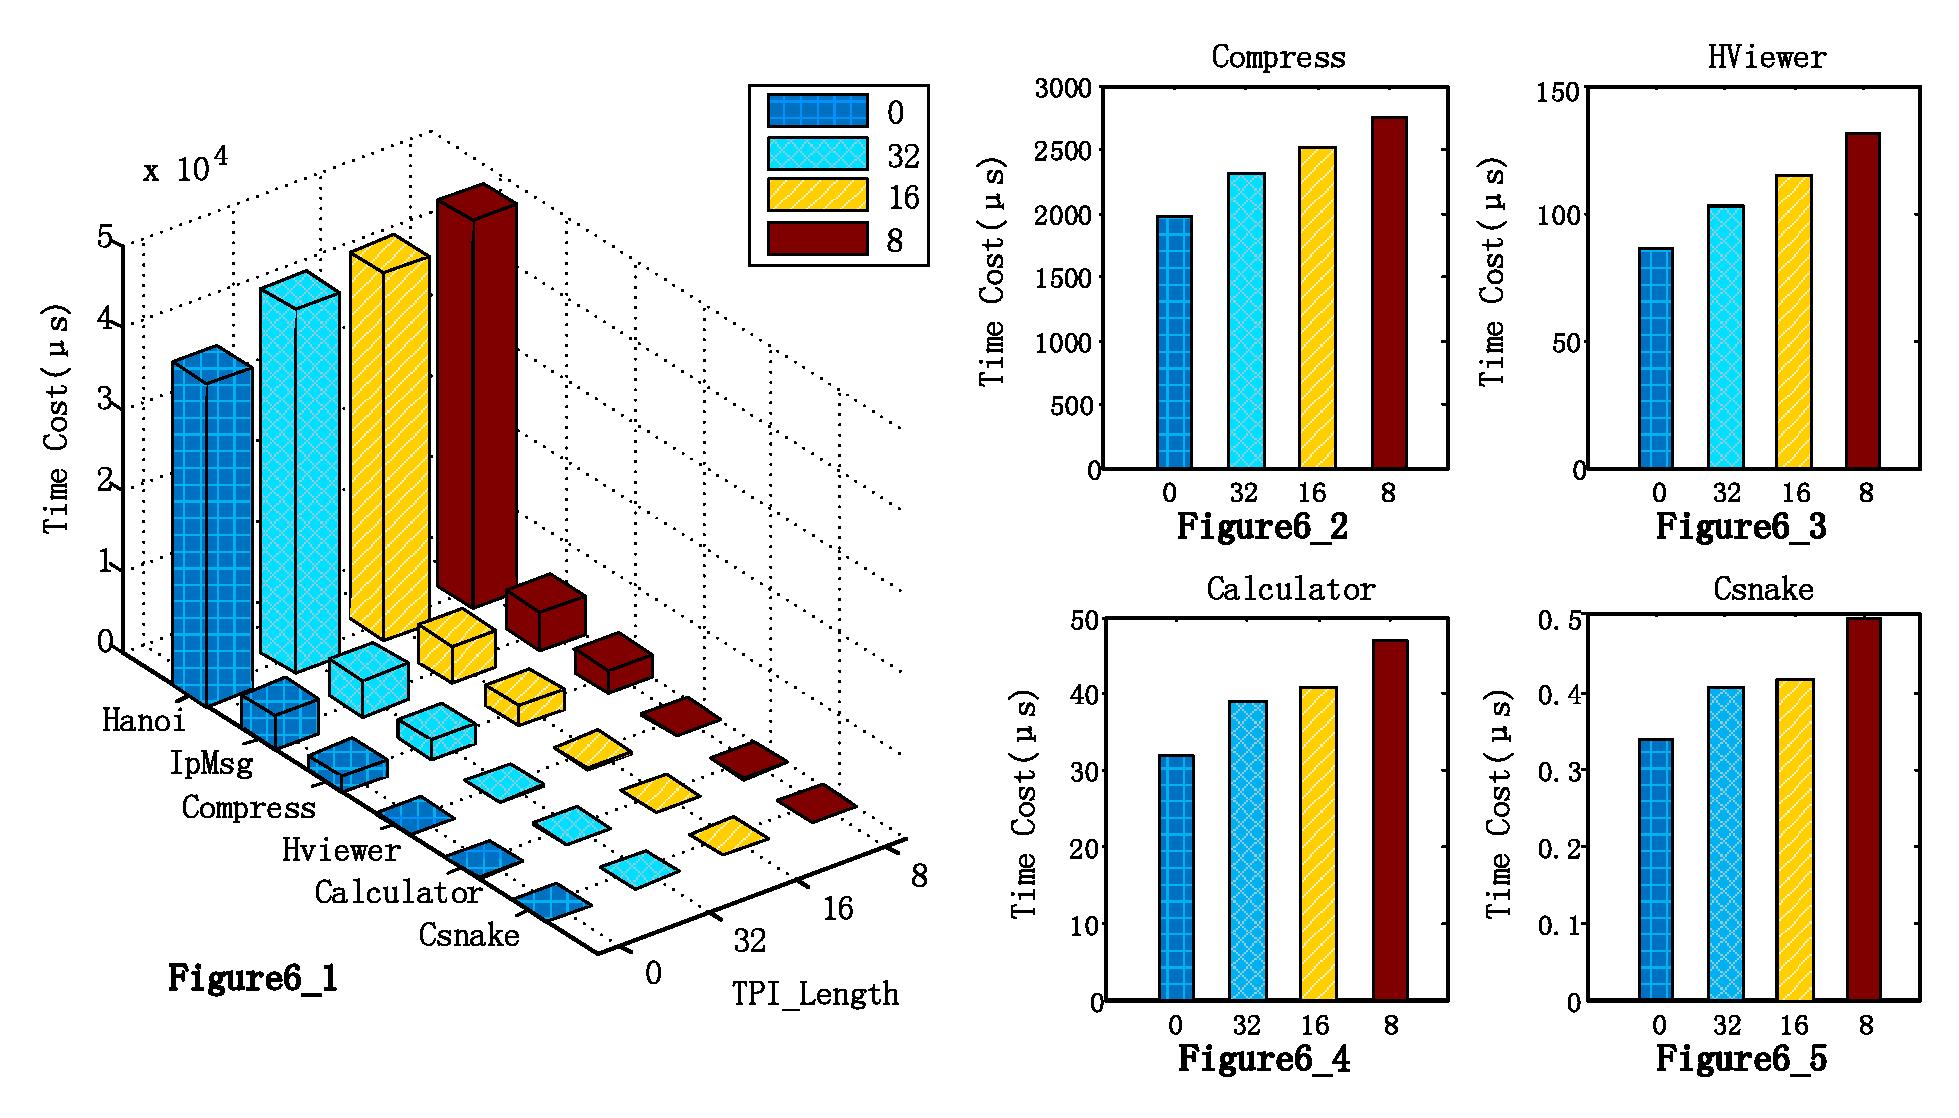
\includegraphics[width=1.0\columnwidth]{figure/runtimeoverhead.pdf}
    \caption{Runtime Overhead}\label{fig:Fig.6}
\end{figure}

Figure~\ref{fig:Fig.6} shows the test results, since different applications, different key-code segment length, different difficulty level of key-code segment, the execution time is obviously different with each other, figure6\_1 represented the all test result, as we can see, it's not clear when we focus on the results of Hviewer, Calculator, and Csnake, so we drew anther four subfigure, figure6\_2 shows the test result of Compress, and figure6\_3 to Hviewer, figure6\_4 to Calculator, figure6\_5 to Csnake. Table3 shows the test result in detail. Take IpMsg.exe as an example, when TPI length is 0, that's to say, we didn't insert any TPI Handler into the protection area, the execution time correspond to the original one. To be clear, we collected 20 different execution time and calculate the average value, so when TPI length is 32 bytes (means the protection range is 32 bytes), the average execution time of the key-code segment is 4462��s, in the same way, when TPI length is 16 bytes and 8 bytes, the average execution times are 4557\textmu s and 4761\textmu s.

%table4
\begin{table}[htb]
\centering
\caption{Execution Time (\textmu s) of different TPI Length}
\begin{tabular}{c|c|c|c|c}
\hline
           & 0     & 32    & 16     & 8      \\ \hline
Hanoi      & 39750 & 44876 & 45268  & 47630  \\ \hline
IpMsg      & 4139  & 4462  & 4557	& 4761 \\ \hline
Compress   & 1970  & 2315  & 2516	& 2760  \\ \hline
HViewer    & 86	   & 103   & 115	& 131\\ \hline
Calculator & 32	   & 39	   & 41	    & 47 \\ \hline
Csnake     & 0.34  & 0.41  & 0.44	& 0.5  \\ \hline
\end{tabular}
\end{table}

In order to see the execution time increment transparently, we defined:

\begin{equation}
  T\_Incre_{rate}= \Delta Time / O\_Time
\end{equation}

We used the formula to calculate an increment for different TPI length. From Figure~\ref{fig:Fig.7}, as the same, we taked IpMsg.exe as an example, when TPI length is 32 bytes, the increment is 7.8\%,when TPI length are 16 bytes and 8 bytes, the increment are 10.1\% and 15.02\% separately. Pay attention, the unit of time is microsecond(\textmu s). You cannot even ``feel'', the application is finished execution.

That's to say, the TPI Handlers we designed are practically useful and time consuming is tolerable. And by default, we set TPI length to 16 bytes, as we can see that when TPI length is 16 bytes, the increment of execution time is around 17\%. Obviously, 16 bytes length is the most reasonable protection range.

%table3
%figure7,figure8
\begin{figure*}[htb]
\centering
\begin{minipage}[b]{0.5\linewidth}
\centering
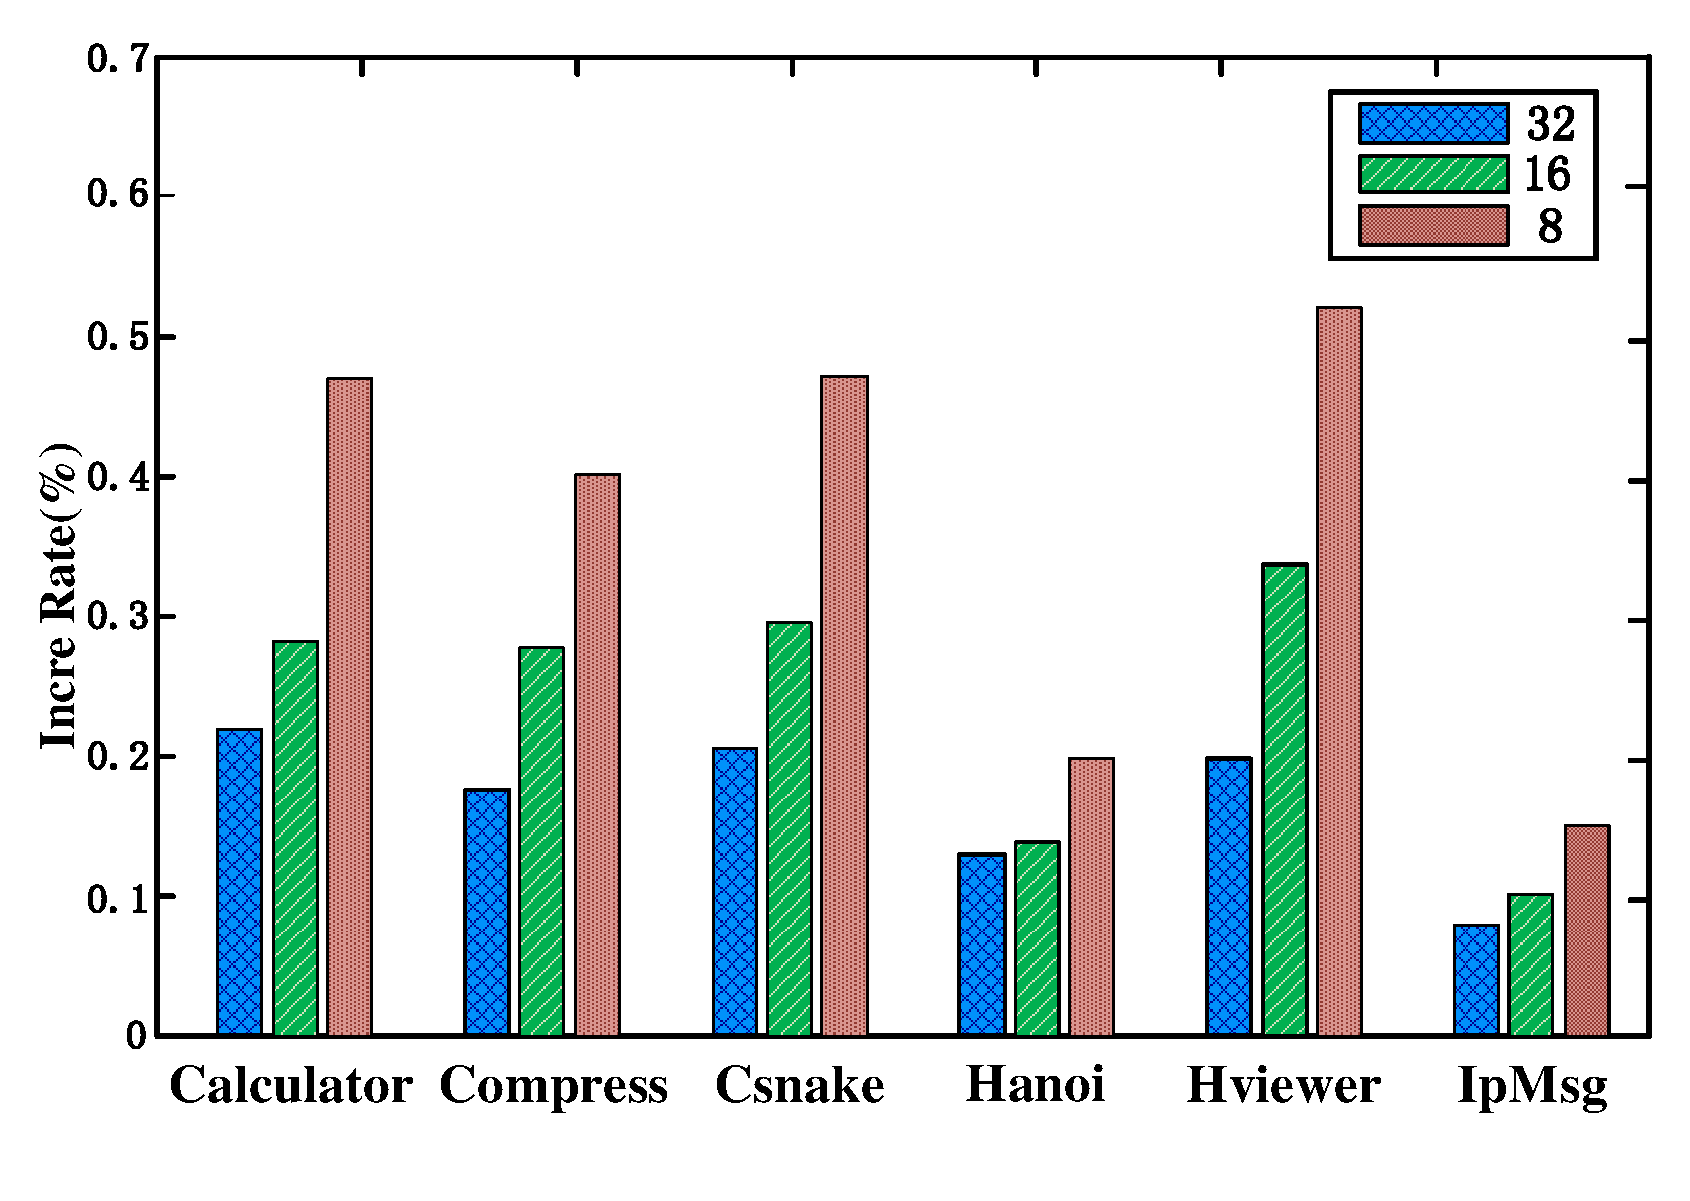
\includegraphics[width=2.3in]{figure/runtime_rate.pdf}
\captionsetup{justification=centering}
\caption{Increment of different\protect\\
 length of TPI}
\label{fig:Fig.7}
\end{minipage}%
\begin{minipage}[b]{0.5\linewidth}
\centering
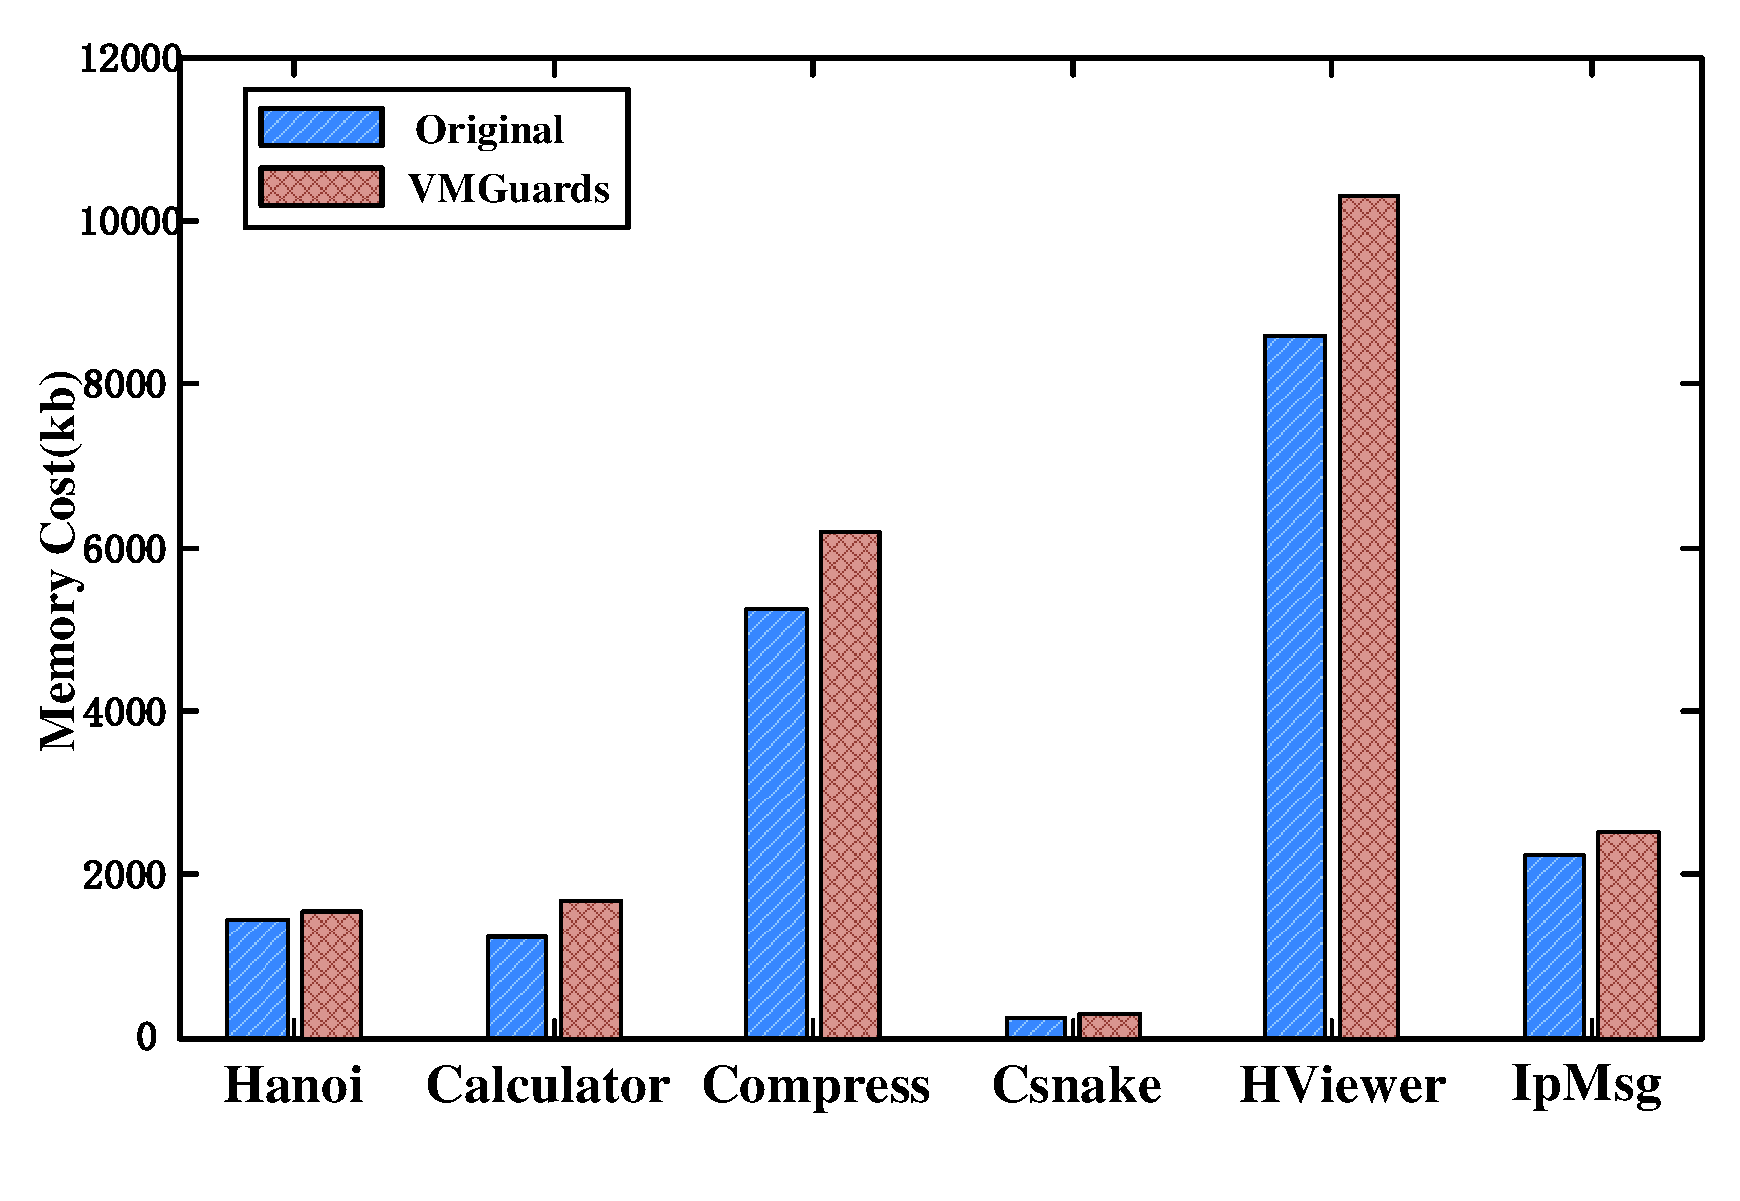
\includegraphics[width=2.3in]{figure/mem_cost.pdf}
\captionsetup{justification=centering}
\caption{Memory cost of the test cases\protect\\
 before and after protected}
\label{fig:Fig.8}
\end{minipage}
\end{figure*}


\subsubsection{Space Overhead}

Our instrumentation adds a new code section to the original program that is on average 1.03 times the original code size. The new section contains more than one Dispatcher to assign Handlers jump to the right addresses to execution. The Dispatchers are mostly like an address translation table for every Handler.

Figure~\ref{fig:Fig.8} shows different applications average running memory costs, the blue bar-graph represented the memory costs when the original programs are running. Correspondingly, the red bar-graph shows the memory costs when the protected programs are running. In total, the space overhead for VMGuards is 117\% over the original program. Note that although the file size has increased, execution must be confined to the new code. Except in the case of programs that store read-only data in their code, other program don't access their code even once. Hence the runtime memory overhead is unaffected by the presence of the original copy of file.

\subsubsection{Performance of VMGuards}

We tested the applications shown in Table2 with commercial software Code Virtualizer1.3.1.0 (short for CV) and VMProtect1.7.0 (short for VMP) compared with our VMGuards.  We set CV to the lowest protection strength, and VMP to the fastest execution time. Figure~\ref{fig:Fig.9} shows the average file size and average execution time change.

%figure9
\begin{figure}[htb]
\centering
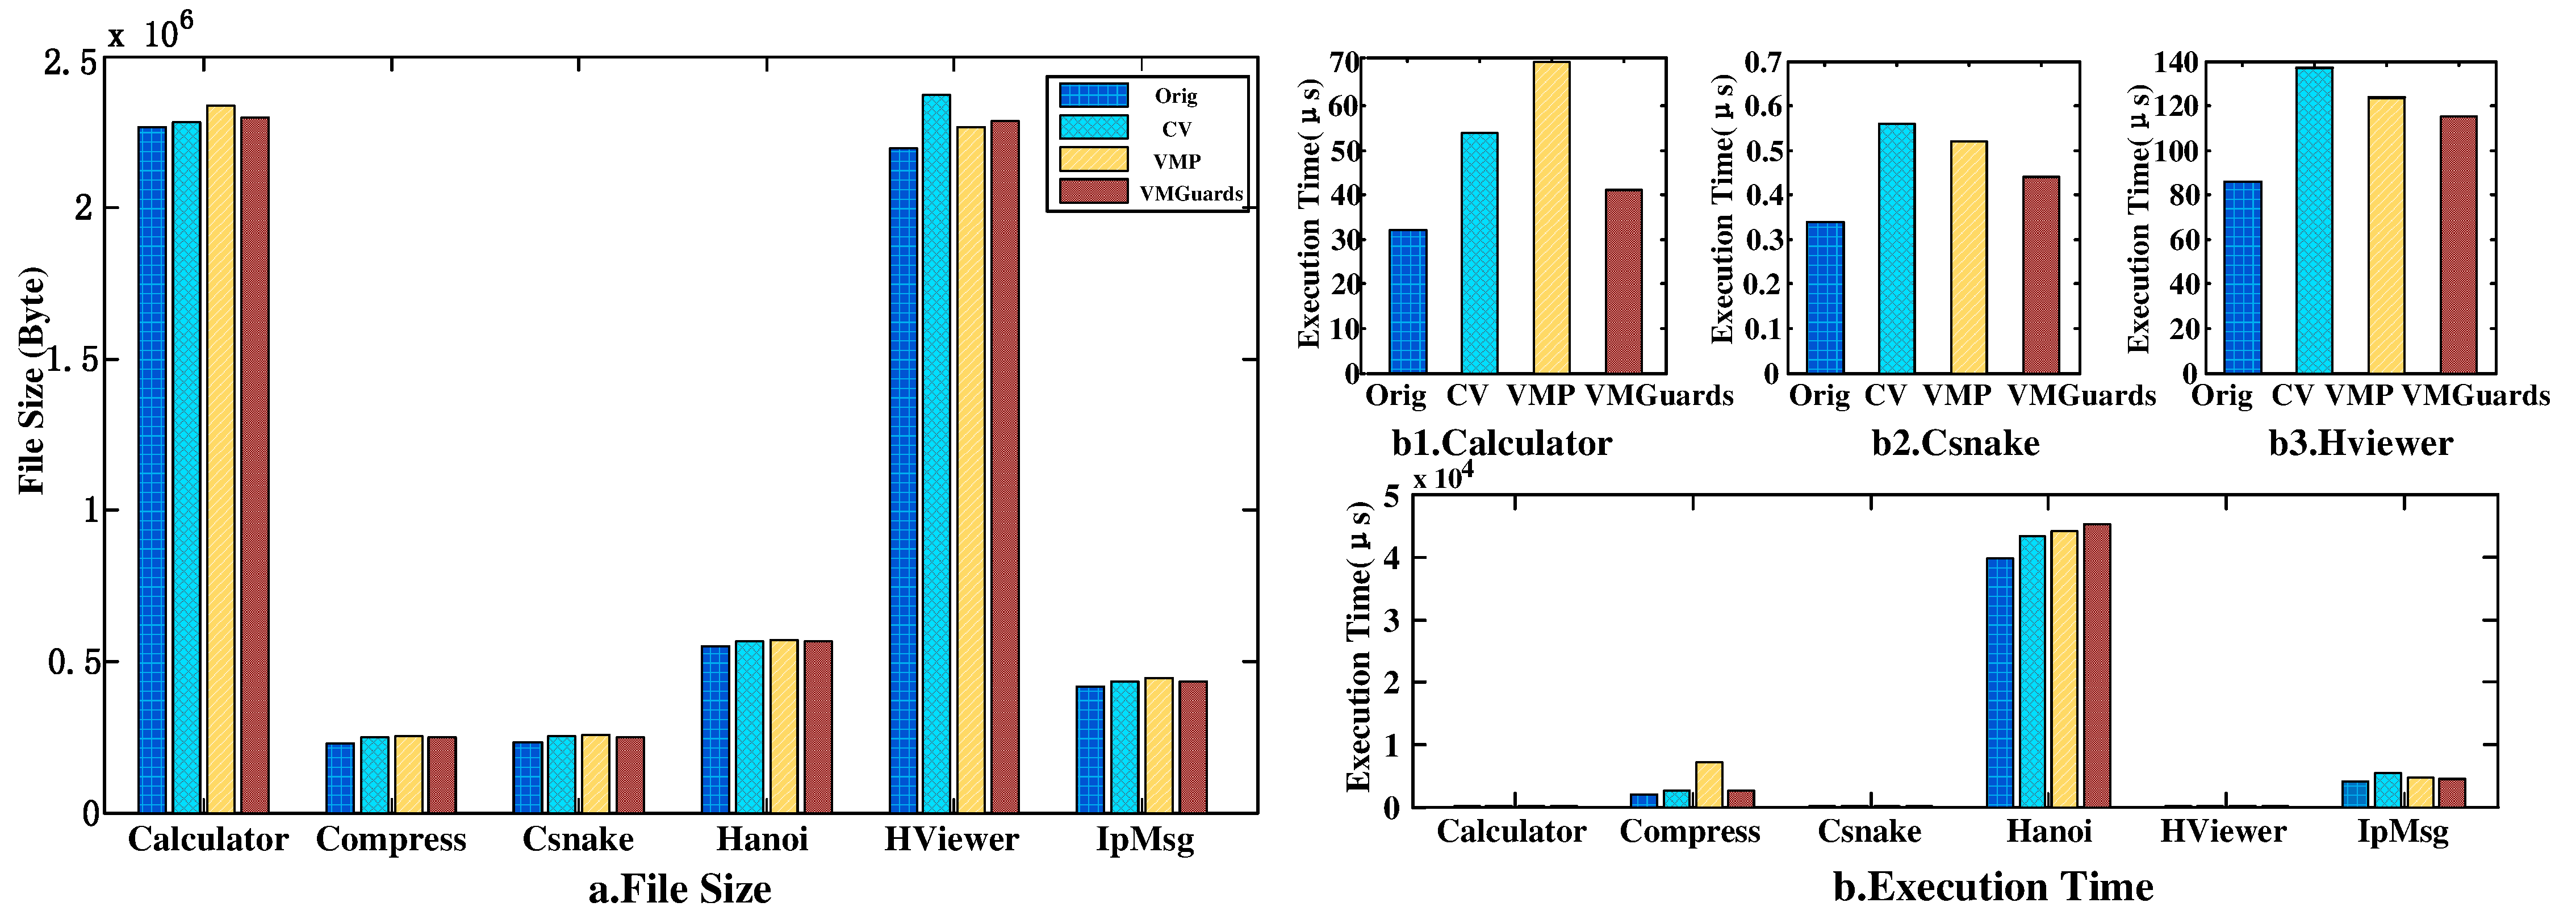
\includegraphics[width=1.0\columnwidth]{figure/filesize_executiontime.pdf}
\captionsetup{justification=centering}
\caption{File Size and Execution Time Differences compared different commercial PVM with our VMGuards}
\label{fig:Fig.9}
\end{figure}


As we can see from Figure~\ref{fig:Fig.9}, comparing with commercial software, our VMGuards does not extra increase the space overhead. However, about runtime overhead, our VMGuards showed some unstable results.

Reasons can be, a) x86 instruction whether it's different type or different address model, when VMGuards, as we described before, is interpreting execution, Handler sequences used to interpret VI are different from each other, b) there still exist some x86 instructions cannot be interpreted by existing Handlers, program needs to retreat from VMGuards, executing the x86 instruction by host machine then back to VMGuards, continue interpreting execution the left VI. Thus, the runtime overhead can be huge, c) owing to the design of multiple Dispatchers, execution time to different instances can be short or long, and we need to further study on it.

\subsection{Case Study}

Our VMGuards, in fact, is an improved Process-Level Machine, which mainly focuses on improve the security of PVM through two security instructions, Tamper-proofing instruction (TPI) and Anti-debug instruction (ADI). Most evaluations are based on theoretical analysis, since there is not a standard when come to evaluate the security of software protection techniques. We will evaluate the security of TPI and ADI through both experiments and theoretical.

Additionally, we had 20 people as a group who knew the basic framework of VMGuards, but did not know the improved points, and another 20 people interest in crack programs to help us experiment the security of TPI and ADI through their efforts to break the protected test cases mentioned in Table2.

\subsubsection{Security of Tamper-Proofing Instruction}

As described in Section4, we organized our Tamper-Proofing Instruction into a ring. Comparing with guards net, TPI-Ring reduced the space overhead brought by complex network theoretically. However, TPI Handlers in TPI-ring didn't lower the self-security of TPI Handlers. We can also see from Figure~\ref{fig:Fig.4} that every TPI Handler is crossed with each other. In another word, there are at least 3 TPI Handlers protecting one address segment when the protected program is running. Stand by the adversary's side, when he tries to break the TPI-Ring, unless he can remove all the TPI Handlers at one time, he would not get what he wants.

In order to clearly see the TPI-Ring, we did some modification to re-organize and centralize the whole function TPI's three handler together. Based on some reverse-engineering experiences, we found three sets TPIs which deployed in the virtual instructions. See from Table4.
\newline

\makeatletter\def\@captype{table}\makeatother
\begin{minipage}[b]{0.45\linewidth}
\flushleft
\begin{tabular}{|c|c|c|}
\hline
\textbf{0043E2E4} & AD 33 C3 05 & DB  04 20  5F \\ \hline
\textbf{0043E2EC} &\color{blue}{2D 23 6E A0} & \color{blue}{6F 2B D8 66} \\ \hline
\textbf{0043E2F4} &\color{blue}{8B 14 24 52} & \color{blue}{8B D4 83 C2} \\ \hline
\textbf{0043E2FC} & 04 83 C2  02 & 87  14 24 8B \\ \hline
\end{tabular}
\caption{TPI protected area.}
\end{minipage}%
\makeatletter\def\@captype{figure}\makeatother
\begin{minipage}[b]{0.54\linewidth}
\centering
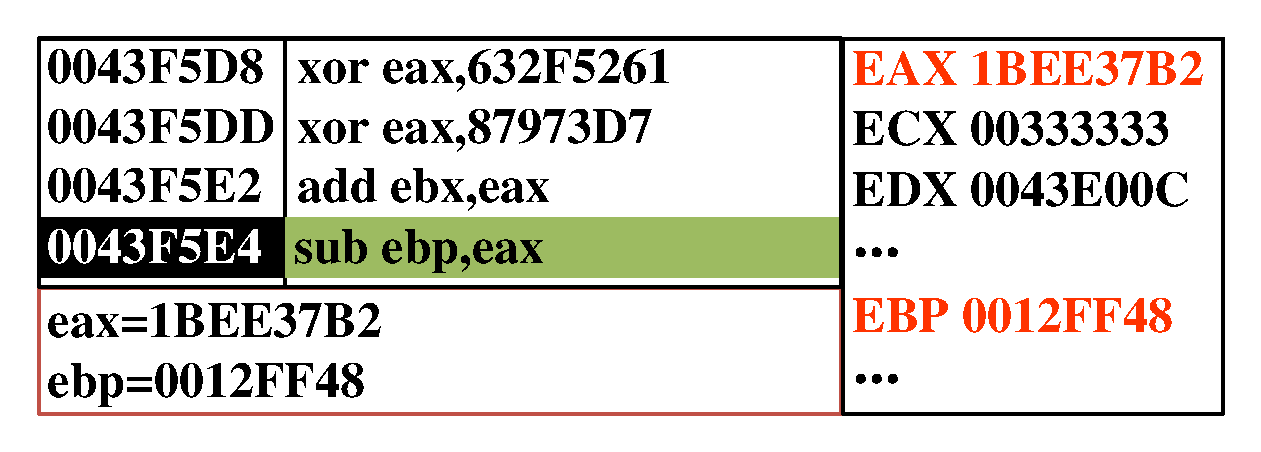
\includegraphics[width=2.0in]{figure/10.pdf}
\caption{Part of Original TPI Handler}
\label{fig:Fig.10}
\end{minipage}
%figure10

As described in section 6.1, we set the length of TPI to 16 bytes.  Based on the idea of cross protection, the start addresses and the end addresses of the three sets TPI are 0043E2E4-0043E2F4, 00E3E2EC-0043E2FC, and 0043E2F4-0043E304. For demonstration, we employed a simple checksum algorithm, add the data of the protection range with 4 bytes length up together. During program execution, it will loop to re-compute a checksum1 from the start address to the end address. If we assume that we choose the second set of TPI to test the functionality, firstly, TPI\_a will decrypt out a checksum (1BEE37B2), then TPI\_b and TPI\_c will find the start address (00E3E2EC) and the end address (0043E2FC). Figure~\ref{fig:Fig.10} is a part of original TPI Handler.

Here is our spark point comparing the normal checksum algorithm, as we know, the value of a register will be frequently invoked during program execution, we didn't just simply compare the pre\_checksum with the checksum re-calculated during the program execution, but minus the pre\_checksum with the value of a register (EBP), loop accumulating to restore the value of EBP, see figure~\ref{fig:Fig.11}. If the value of EBP is not changed, there is no tamper occurred, otherwise, the program will be crashed when it comes to invoke EBP.

%figure11
\begin{figure*}[htb]
\centering
\begin{minipage}[b]{0.5\linewidth}
\centering
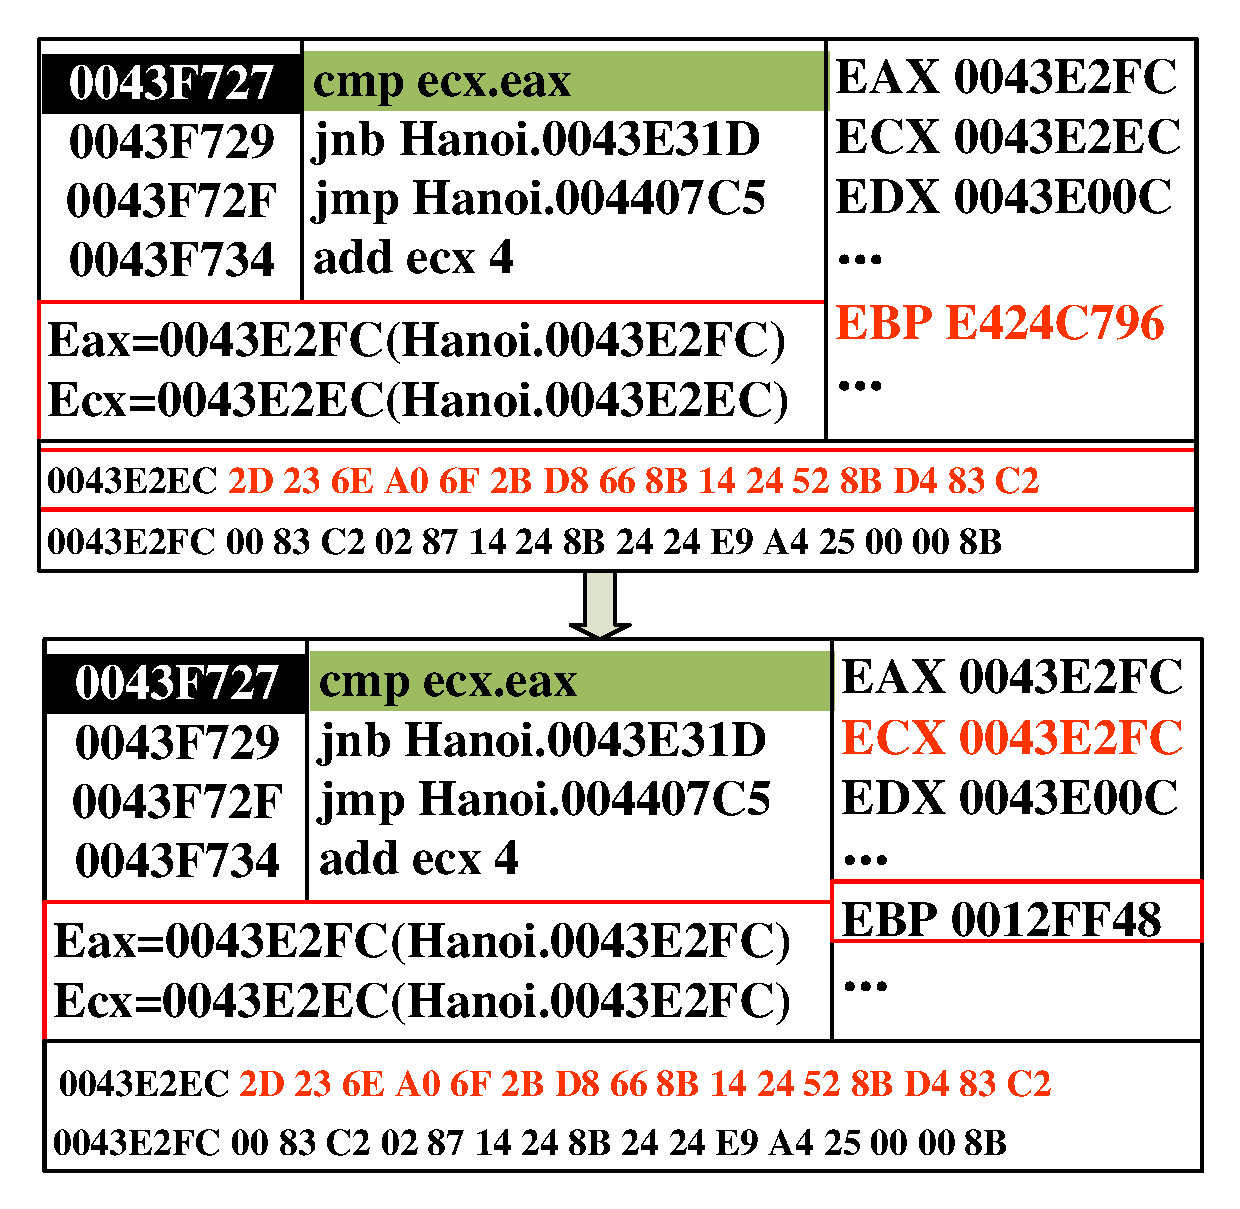
\includegraphics[width=2.4in]{figure/11.pdf}
\captionsetup{justification=centering}
\caption{Sample of Tamper-Proofing Instruction\\  }
\label{fig:Fig.11}
\end{minipage}%
\begin{minipage}[b]{0.5\linewidth}
\centering
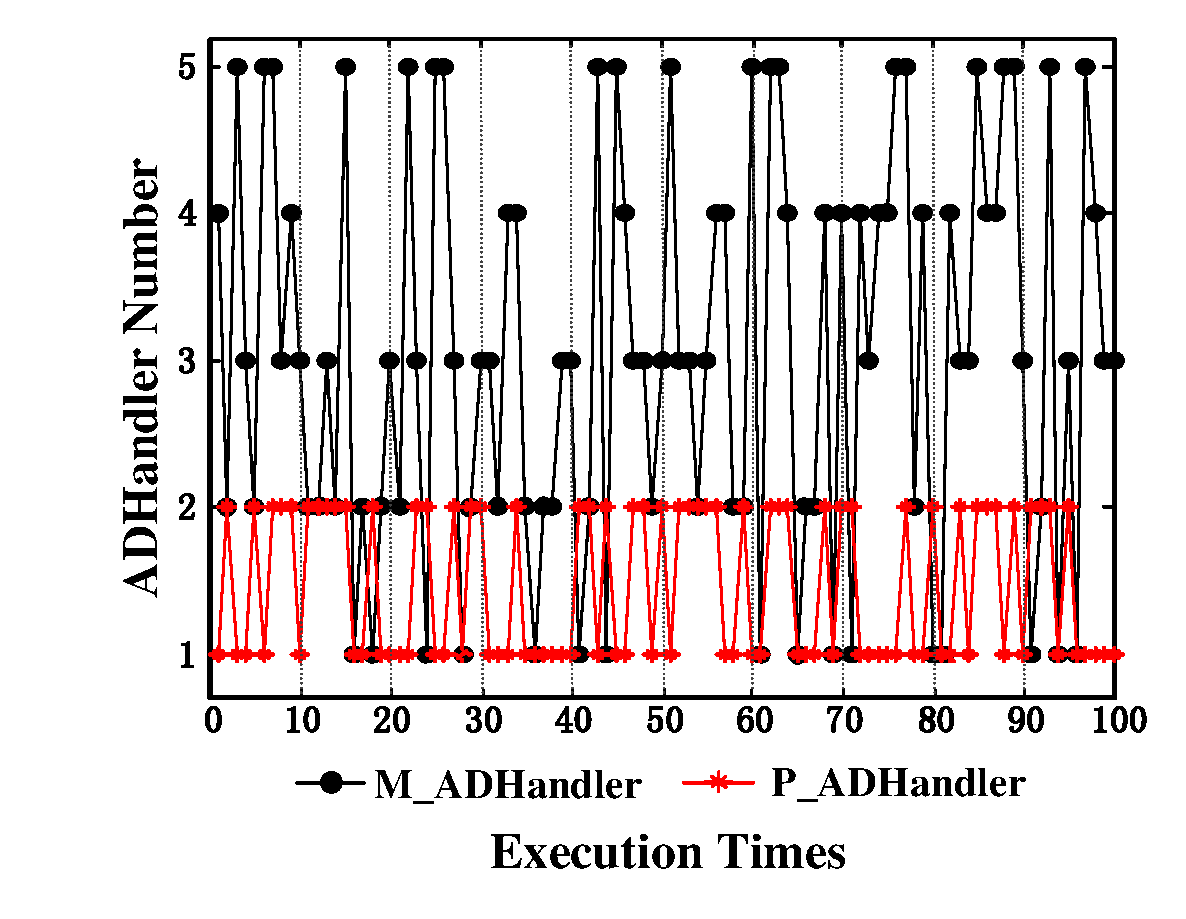
\includegraphics[width=2.3in]{figure/14.pdf}
\captionsetup{justification=centering}
\caption{Statistics result in 100 times executions, M for Monitor Handler, P for Process Handler}
\label{fig:Fig.14}
\end{minipage}
\end{figure*}


Theoretically, if we modified some data within the second TPI's protection range, we believe that not only the three TPIs, but also the whole TPI-ring can aware the tamper behavior.

\subsubsection{Effectiveness of Anti-Debug Instruction}

Assuming that Tamper Proofing Instructions prevent the program itself from modifying, we applied Anti-Debug Instruction to guarantee that the execution environment of the program is harmless. As described in Section5, we designed seven anti-debug security instructions, that's to say, we designed seven different Handlers to achieve the goal of all these anti-debug instructions.

%figure12
%figure13
\begin{figure*}[htb]
\centering
\begin{minipage}[b]{0.5\linewidth}
\centering
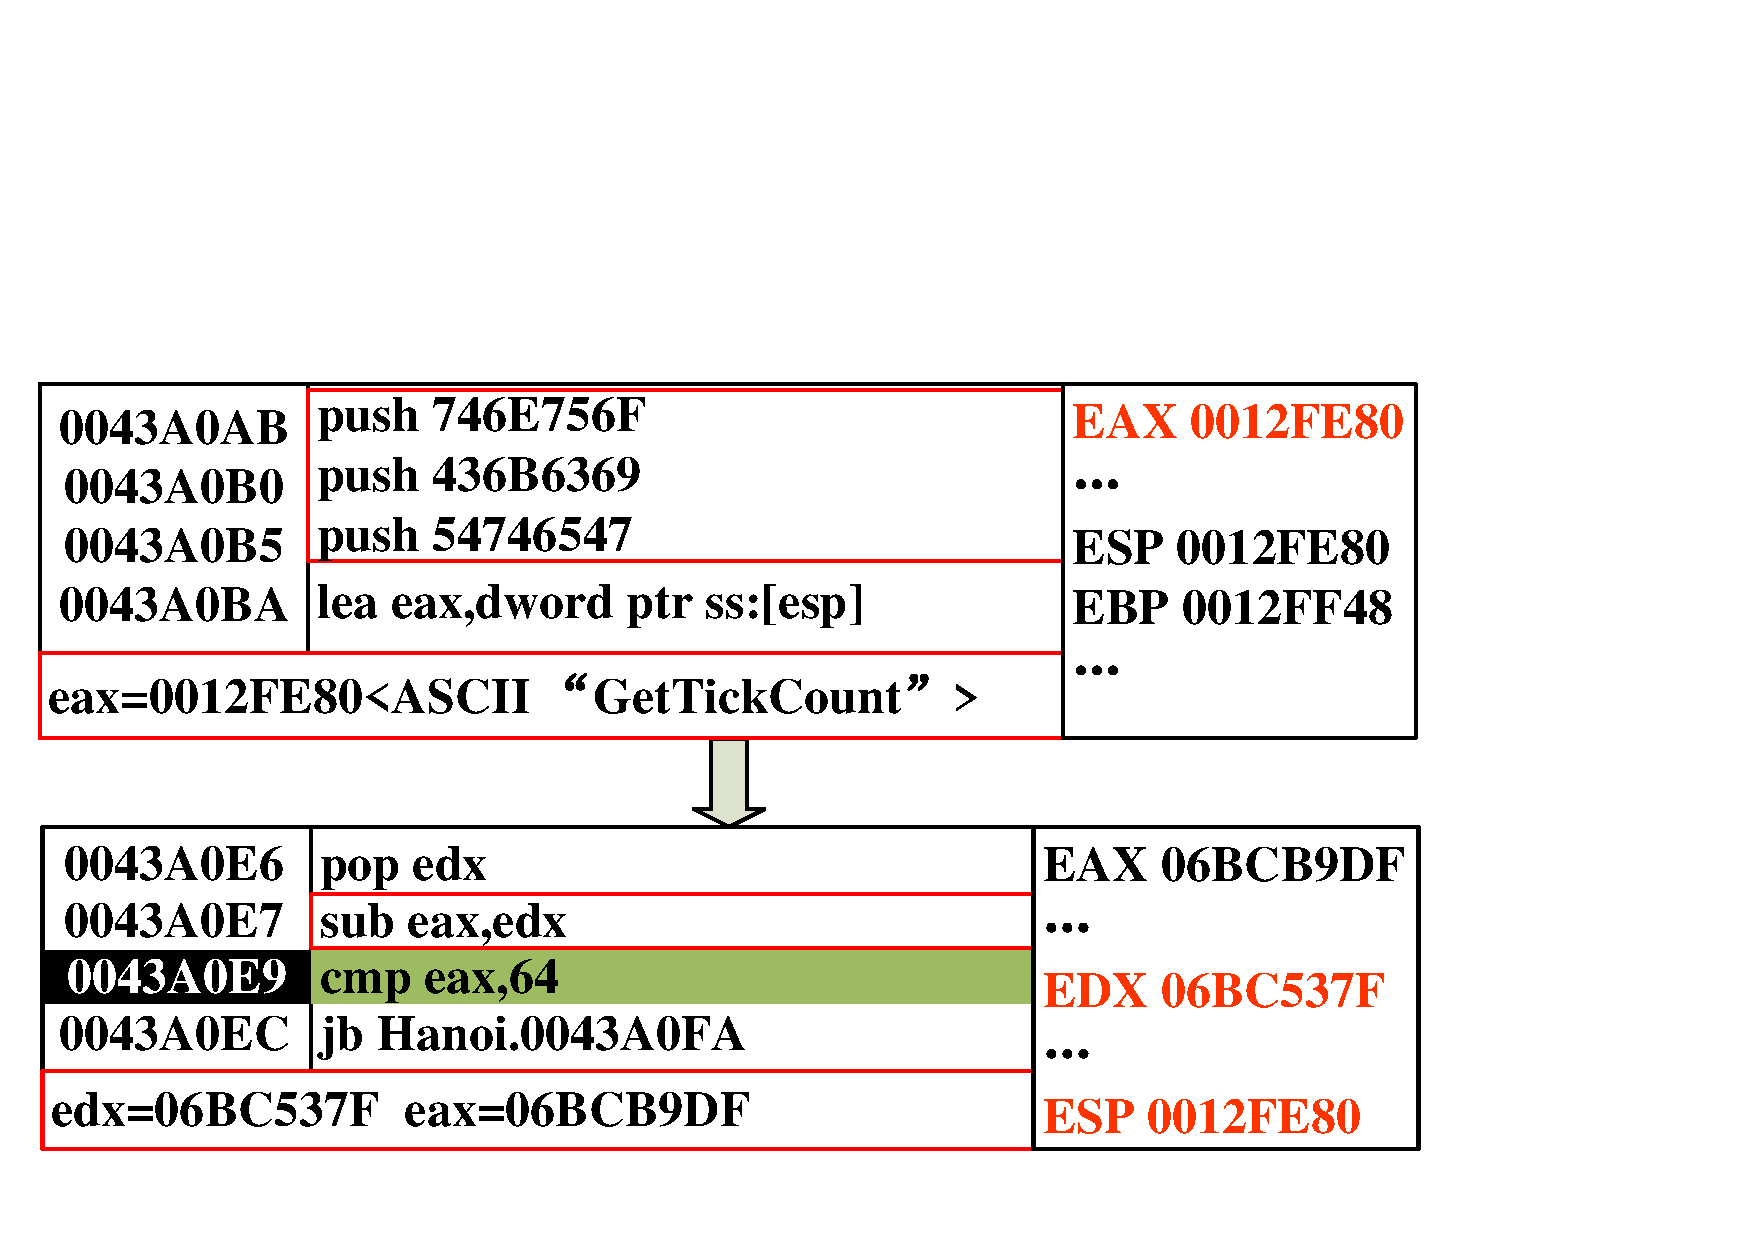
\includegraphics[width=2.2in]{figure/12.pdf}
\captionsetup{justification=centering}
\caption{Sample of Monitoring ADHandler}
\label{fig:Fig.12}
\end{minipage}%
\begin{minipage}[b]{0.5\linewidth}
\centering
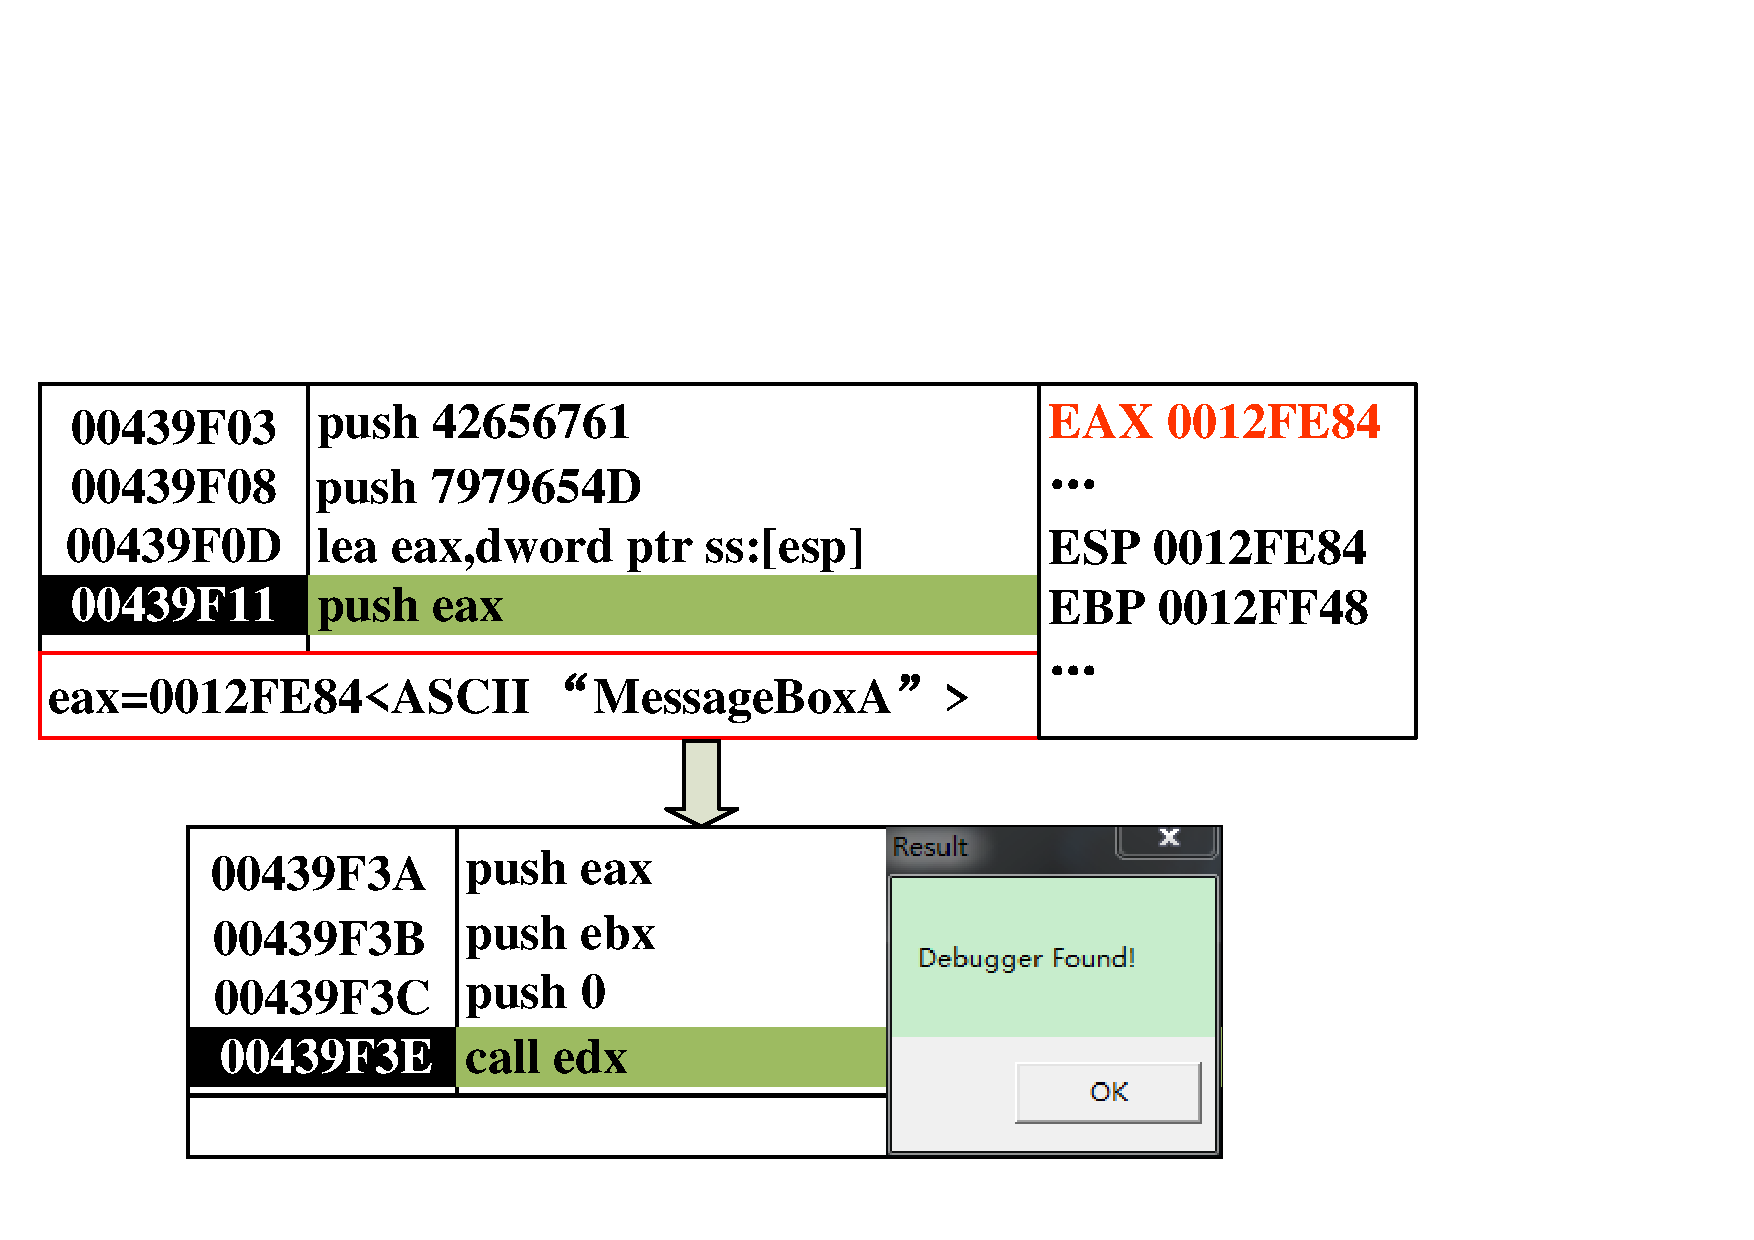
\includegraphics[width=2.2in]{figure/13.pdf}
\captionsetup{justification=centering}
\caption{Sample of Processing ADHandler}
\label{fig:Fig.13}
\end{minipage}
\end{figure*}

Experimentally, VMGuards randomly chose the Execution\_Time\_Difference monitor Handler to detect whether the program is being debugged during protection procedure, as we can see from Figure~\ref{fig:Fig.12}.

Processing Handler will be chosen to respond to the monited debugging behavior, see from Figure~\ref{fig:Fig.13}. The MessageBox Handler was chosen to respond to the Execution\_Time\_Difference Handler.

In every execution, the program will randomly choose one of the five monitor ADI Handler to detect, for example, whether the program under the condition that there is a debugger attacked to itself, or the execution time differences are so different. If the chosen executed monitor ADI is happen to be detected, then the program will randomly choose one of the two processing ADI to alter user that the program is being debugged with a MessageBox or just terminate the program roughly.


%figure14


Figure~\ref{fig:Fig.14} shows 100 times the execution results of the protected program. As mentioned before, which monitor Handler and Processing Handler will be chosen to execution are all depend on the random number, as a result, the statistics results are not inexorable law to follow.

\subsection{Discussion}

This section states some of the protective aspects of the VMGuards, as well as vulnerabilities inherent to PVM-based security measures.

\subsubsection{Protection of Virtual Instruction}

The primary goal of Tamper-Proofing Instruction involves protecting the virtual instruction from tamper. To our knowledge, VMGuards is the first PVM-based scheme attempt at tamper-proofing software code. Previously, the adversary could, for instance, locate the critical component-Dispatcher, collect information of all Handlers, and make modifications to the virtual instructions. TPI-Ring can guard all the virtual instructions from tampering, as any changes made by adversary will be detected and responded appropriately. However, over-stress the intensive of TPI adds a serious performance to both runtime and space. As the same, the structure TPI-Ring itself have already adds an additional layer of protection from tampering. With a better balance between TPI protection range and TPI-Ring, VMGuards still can be effectively used to protection program from tampering.

\subsubsection{Effectiveness against Malicious Host}

Anti-Debug Instruction is designed to make sure that the execution environment of the program is unharmed. Currently, anti-debug techniques can be divide into two categories. One is to check hardware or software debug structure for the presence of debugger state such as breakpoint set. The other is to detect human behavior such as the undesired pause during program execution. An unambiguous rule to distinguish the behavior of debugger is recognized as highly significant for the effectiveness and accuracy of the anti-debug technique. However, one drawback of the current anti-debug mechanisms is that most of them fail to conceal themselves from other processes.  If malware or debuggers perceive that they are monitored by anti-debug schemes, they would try every means to bypass such monitoring or even strike back using anti-anti-debug techniques. Anyhow, applying anti-debug technique into PVM-based software protection still can thwart the malicious behavior of an adversary as long as the host machine is harmless.

\section{Related Works}

\textbf{Software Tamper-Proofing} \hspace{1ex}Software programs are increasingly being used to execute critical tasks. At the same time, their protection against undesired modification is of paramount important. Much research has been done in the field of tamper-proofing. The most classical one is based on the seminal research by Aucsmith\cite{tam}. But in total, program protection techniques can be widely classified into two sides:  hardware and software approaches.

Hardware-based approaches are somewhat monetary cost and basically cannot be circle used, but on the other side, these approaches are more difficult to break. By now, there are many hardware solutions have been proposed to against physical and software attacks. Dongles is a very common device that is distributed along with the copy of the software and can be attacked to a computer. The program will invoke a callback discontinuously from dongles during the execution progress of the program, and if the reply is no sign of abnormal, the program will continue to run, and if not, ceases to run. It's more difficult to debugging the dongles, that's to say, anyone who wants to copy the dongles is illegimate. However, if an adversary can obtain the security function from the dongle, he can also bypass the protection using emulation. Along with the step of time, modern processors possess their own protection functionality in hardware (e.g., the Cell Broadband Engine, which provides the Runtime Secure Boot feature, used to verify an application has not been tampered with at start up\cite{cell}).Other hardware solutions involve the use of trusted computing platforms such as TPM and Microsoft's NGSCB\cite{over}. Finally there are customized hardware techniques to prevent tampering, such as execute-only memory\cite{arch} and systems based on secure processors\cite{aeg}.

On the contrast, software-based approaches are used more generally. Chang\cite{prot} proposed the original guards used to tamper-proofing, which employed the idea of checksum guards to protect the integrity of an application. After which, Horne\cite{ind} et al. came up with the concept of tester, which is similar to the guards, consisting of a sequence of instructions that calculated a hash value of  fixed length addresses, during the program runtime, comparing the hash value with a corrector.

Oblivious hashing\cite{tamp,obl} is a tamper-proofing technique that computes hash values based on the real execution path of the application. Owing to the vulnerabilities of static checksums\cite{gen}, various measurements have been proposed to solve the problems, such as knots\cite{sof}, self-sensing guards\cite{def}.

Obfuscation techniques also have been broadly used to the area of software tamper-proofing to make it troublesome for an adversary to understand and analyse the original code of an application. Collberg et al. provided numbers of obfuscation techniques to obscure the code\cite{man,tax}. Linn et al. designed a novel technique to disturb the disassembly of the code\cite{obfu}. Wang et al. proposed the use of indirect branches to obfuscate the control flow of a program. Encryption the program code is another way to solid the program, the specific hardware can decode the code (i.e., a secure co-processor\cite{appr}), but as we mentioned before, its cost a lot than other software-based approaches. Nevertheless, these static obfuscation techniques is vulnerable to some dynamic analysis techniques\cite{sil}.

\vspace{2ex}
\noindent\textbf{Process-Level Virtual Machine}\hspace{1ex}Among numbers of software-based tamper-proofing techniques, virtualization is a milestone which improved the protection techniques, especially in runtime protection scenario. Currently, a number of commercial PVM have been created, such as VMProtect\cite{vmp}, Code Virtualizer\cite{code} and Themida\cite{the}. These tools protect the program using a mid-expression �C Instruction Set Architecture (ISA)\cite{pro} and the code will be interpreted during program run time.

Among the existing research about PVM, almost each of them integrates various protection techniques together. Literature\cite{def} merged the idea of diversity together with virtual machine, proposing a diversity software protection model based on virtual machine. They also designed a software protection RSIC-based virtual machine, it's the first work that merge the diversity with VM; also, literature\cite{mult} introduced the concept of multi-stage binary code obfuscation to obscure a program. It will first proceed n times control flow obfuscation at the beginning of the VM protection��then it will choose the key code segment to be protected, moreover, their work also adopted the centralized and chained dispatching model. This is the first research work to improve the VM's dispatching structure, one basic block a time to serve as the dispatching unit, and combined the multiple-level obfuscation, to furthermore enhance the protection strength of the VM; literature\cite{bus} presented another VM protection method based on adaptive dynamic instruction set, it dug down virtual machine protection mechanism, enhancing the execution efficiency and security of the protected program; literature\cite{def} further merged the virtual junk instruction sequence and virtual instruction obscure transformation technique together, and moreover it improved the design of virtual instruction set, making it much harder for an adversary to reverse-engineering the protected program. All in all, the research on PVM is much valuable than it appears.

\section{Conclusions}

Taking Process-level Virtual Machine (PVM) as one of software protection technique seems gradually increasing in recent years. In this paper, we presents a novel use of PVMs in the field of temper-proofing, and we designed a proof of concept prototype, we call it VMGuards. VMGuards uses Tamper-Proofing Instruction (TPI, it's similar with the concept of guards proposed by Chang\cite{prot}) to maintain the integrity of the key code segment from malicious modifications. TPI is designed to be similar with the normal Handlers, will be placed in random locations during program creation time. At run time, TPI Handlers will calculate another checksum to compare with the pre\_checksum cached in a virtual register v\_ebp, if the two checksums are equal, there is no tamper occurs, and if not, the program will secretly change the value of the virtual register v\_ebp, next time when v\_ebp is used again, the program will be failed. Furthermore, we introduced the anti-debug techniques when an adversary tries to debug the protected program, the program will know that there is a debugger exist in the host compute, then the program will take some respond measurements. The experiment results indicate that our VMGuards can provide a good balance between execution rate and overhead, and moreover provide a platform for different program protection techniques.

\section{Acknowledgment}

This work was supported by project National Natural Science Foundation of China (No. 61373177, and No. 61572402),the Key Project of Chinese Ministry of Education (No.211181), the International Cooperation Foundation of Shaanxi Province, China (No. 2013KW01-02, No. 2015KW-003 and No. 2016KW-034), the China Postdoctoral Science Foundation(grant No. 2012M521797), the Research Project of Shaanxi Province Department of Education (No. 15JK1734), and the Research Project of NWU, China (No. 14NW28).


\bibliographystyle{unsrt}
\bibliography{reference}

\end{document}
